\documentclass[11pt,a4paper]{article}
\usepackage[spanish,es-nodecimaldot]{babel}	% Utilizar español
\usepackage[utf8]{inputenc}					% Caracteres UTF-8
\usepackage{graphicx}						% Imagenes
\usepackage[hidelinks]{hyperref}			% Poner enlaces sin marcarlos en rojo
\usepackage{fancyhdr}						% Modificar encabezados y pies de pagina
\usepackage{float}							% Insertar figuras
\usepackage[textwidth=395pt]{geometry}		% Anchura de la pagina
\usepackage[nottoc]{tocbibind}				% Referencias (no incluir num pagina indice en Indice)
\usepackage{enumitem}						% Permitir enumerate con distintos simbolos
\usepackage[T1]{fontenc}					% Usar textsc en sections
\usepackage{amsmath}						% Símbolos matemáticos
\usepackage{algorithm}						% Environtment algorithm
\usepackage[noend]{algpseudocode}			% Pseudocodigo
\usepackage{listings}

\algnewcommand\algorithmicforeach{\textbf{for each}}
\algdef{S}[FOR]{ForEach}[1]{\algorithmicforeach\ #1\ \algorithmicdo}

\algrenewcommand\algorithmicreturn{\textbf{return}}


\lstset{
	language=bash
}

% Comando para poner el nombre de la asignatura
\newcommand{\asignatura}{Metaheurísticas}
\newcommand{\autor}{Vladislav Nikolov Vasilev}

% Configuracion de encabezados y pies de pagina
\pagestyle{fancy}
\lhead{\autor{}}
\rhead{\asignatura{}}
\lfoot{Grado en Ingeniería Informática}
\cfoot{}
\rfoot{\thepage}
\renewcommand{\headrulewidth}{0.4pt}		% Linea cabeza de pagina
\renewcommand{\footrulewidth}{0.4pt}		% Linea pie de pagina

\begin{document}
\pagenumbering{gobble}

% Pagina de titulo
\begin{titlepage}

\begin{minipage}{\textwidth}

\centering

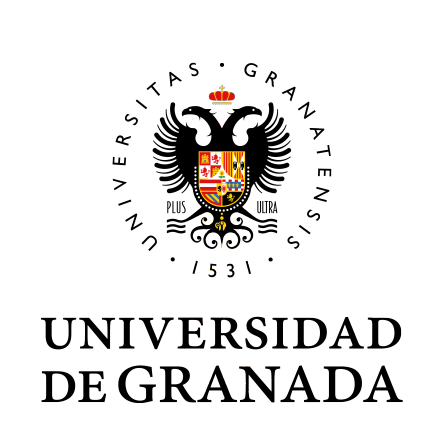
\includegraphics[scale=0.3]{img/ugr.png}\\

\textsc{\Large \asignatura{}\\[0.2cm]}
\textsc{GRADO EN INGENIERÍA INFORMÁTICA}\\[0.3cm]

\noindent\rule[-1ex]{\textwidth}{1pt}\\[1.5ex]
\textsc{{\Huge PRÁCTICA 2\\[1pt]}}
\textsc{{\Large \\Técnicas de Búsqueda basadas en Poblaciones para el Problema del Aprendizaje de Pesos en Características}}
\noindent\rule[-1ex]{\textwidth}{2pt}\\[1ex]

\end{minipage}

\vspace{0.18cm}

\begin{minipage}{\textwidth}

\centering

\textbf{Autor}\\ {\autor{}}\\[1ex]
\textbf{NIE}\\ {X8743846M}\\[1ex]
\textbf{E-Mail}\\ {vladis890@gmail.com}\\[1ex]
\textbf{Grupo de prácticas}\\ {MH3 Jueves 17:30-19:30}\\[1ex]
\textbf{Rama}\\ {Computación y Sistemas Inteligentes}\\[1ex]
\vspace{0.2cm}


\includegraphics[scale=0.3]{img/etsiit.jpeg}

\vspace{0.3cm}
\textsc{Escuela Técnica Superior de Ingenierías Informática y de Telecomunicación}\\
\vspace{1cm}
\textsc{Curso 2018-2019}
\end{minipage}
\end{titlepage}

\pagenumbering{arabic}
\tableofcontents
\thispagestyle{empty}				% No usar estilo en la pagina de indice

\newpage

\setlength{\parskip}{1em}

\section{Descripción del problema}

El problema que se aborda en esta práctica es el Aprendizaje de Pesos en Características (APC). Es un problema típico de
\textit{machine learning} en el cuál se pretende optimizar el rendimiento de un clasificador basado en vecinos más cercanos.
Esto se consigue mediante la ponderación de las características de entrada con un vector de pesos $W$, el cuál utiliza
codificación real (cada $w_i \in W$ es un número real), con el objetivo de modificar sus valores a la hora de calcular la
distancia. Cada vector $W$ se expresa como $W = \lbrace w_1, w_2, \dots , w_n \rbrace$, siendo $n$ el número de dimensiones
del vector de características, y cumpliéndose además que $\forall w_i \in W, \; w_i \in [0, 1]$.\par

El clasificador considerado para este problema es el 1-NN (genéricamente, un clasificador $k$-NN, con $k$ vecinos, siendo
en este caso $k = 1$), es decir, aquél que clasifica un elemento según su primer vecino más cercano utilizando alguna medida
de distancia (en este caso, utilizando la distancia Euclídea). Cabe destacar que no en todos los casos se usará el clasificador
1-NN ya que se pueden dar casos en los que el vecino más cercano de un elemento sea él mismo. Por ese motivo, en algunas
técnicas/algoritmos se usará un 1-NN con el criterio de \textit{leave-one-out}, es decir, que se busca el vecino más cercano
pero excluyéndose a él mismo.\par

El objetivo propuesto es aprender el vector de pesos $W$
mediante una serie de algoritmos, de tal forma que al optimizar el clasificador se mejore tanto la precisión de éste como su
complejidad, es decir, que se considere un menor número de características. Estos dos parámetros, a los que llamaremos $tasa\_
clas$ y $tasa\_red$, respectivamente, se pueden expresar de la siguiente forma:

\[tasa\_clas = 100 \cdot \frac{nº \; instancias \; bien \; clasificadas \; en \; T}{nº \; instancias \; en \; T}\]
\[tasa\_red = 100 \cdot \frac{nº \; valores \; w_i < 0.2}{nº \; caracteristicas}\]

\noindent siendo $T$ el tamaño del conjunto de datos sobre que el que se evalúa el clasificador.\par

Por tanto, al combinarlos en una única función a la que llamaremos $F(W)$, la cuál será nuestra función objetivo a optimizar
(maximizar), tenemos que:

\[F(W) = \alpha \cdot tasa\_clas(W) + (1 - \alpha) \cdot tasa\_red(W)\] 

\noindent siendo $\alpha$ la importancia que se le asigna a la tasa de clasificación y a la de reducción, cumpliendo que
$\alpha \in [0, 1]$. En este caso, se utiliza un $\alpha = 0.5$ para dar la misma importancia a ambos, con lo cuál se pretende
que se reduzcan al máximo el número de características conservando una $tasa\_clas$ alta.

\section{Descripción de los algoritmos}

\subsection{Consideraciones previas}

Antes de empezar con la descripción formal de los algoritmos implementados, vamos a describir algunos aspectos
comunes, como por ejemplo cómo se representan e inicializan las soluciones; cómo se representan la población, los padres y las
elecciones para mutar los cromosomas; cómo se realiza el torneo binario, la mutación y los distintos cruces, y algunas funciones
utilizadas en muchas partes del código, como por ejemplo la función objetivo o la forma de evaluar a la población. Cabe destacar
que muchos de los pseudocódigos que aparecen a continuación no se han implementado exactamente igual o no aparecen en el
código, ya que o bien son operaciones que se han vectorizado o bien ya hay funciones que hacen eso.

Primero vamos a ver como se representa la población, los padres y una elección de mutación. Una población no es más que un
vector de vectores, o lo que es lo mismo, una matriz de tamaño $N \times M$, donde $N$ es el número de cromosomas (soluciones)
y $M$ es el número de genes (número de características). Por tanto, ahora tenemos un conjunto de vectores de pesos, lo que
viene a significar que tenemos múltiples $W$. Esta población está ordenada en todo momento por el valor \textit{fitness}
de cada cromosoma para facilitar las operaciones posteriores. Un padre $p$ no es más que un índice de un cromosoma de la
población, con la restricción de que $p \in [0, N)$. Una mutación viene dada por dos valores $c, g$, donde $c$ es el cromosoma
a mutar y $g$ el gen a mutar. Estos dos valores están sujetos a que $c \in [0, N)$ y a que $g \in [0, M)$.

Como cada fila de la matriz es un vector de pesos $W$, se tiene que cumplir que $\forall w_i \in W, \; w_i \in [0, 1]$. Por
tanto, para evitar que las soluciones se salgan de este intervalo, se ha implementado una función que se encarga de normalizar
los valores de $W$ en el rango. La función se ha usado tanto en los algoritmos meméticos como en los genéticos a
la hora de realizar un cruce o una mutación, para que los valores de los cromosomas siguiesen siendo válidos. La
implementación de esta función es la siguiente:

\begin{algorithm}[H]
\caption{Función que normaliza un vector de pesos $W$}
\begin{algorithmic}[1]
\Function{NormalizarW}{$W$}
\ForEach{$w_i \in W$}
	\If{$w_i < 0$}
		\State $w_i \gets 0$
	\ElsIf{$w_1 > 1$}
		\State $w_i \gets 1$
	\EndIf
\EndFor
\State \Return{$W$}
\EndFunction
\end{algorithmic}
\end{algorithm}

Para generar las soluciones iniciales se ha utilizado una función que recibe como parámetros el número de genes y el número de
cromosomas, y crea una nueva matriz que representa la población, inicializándola con valores aleatorios generados
mediante una distribución uniforme en el rango $[0, 1]$. Su pseudocódigo se puede ver a continuación:

\begin{algorithm}[H]
\caption{Función que genera una población inicial}
\begin{algorithmic}[1]
\Function{GenerarPoblacionInicial}{$numCrom$, $numGenes$}
\State $poblacion \gets $ NuevaMatrizVacia($numCrom$, $numGenes$)
	\For{$i \gets 0$ \textbf{to} $numCrom - 1$}
		\For{$j \gets 0$ \textbf{to} $numGenes- 1$}
			\State $poblacion[i][j] \gets $ ValorAleatorioUniformeRango0-1()
		\EndFor	
	\EndFor
\State \Return{$poblacion$}
\EndFunction
\end{algorithmic}
\end{algorithm}

Para seleccionar los padres o cromosomas que pasarán su material genético se ha utilizado una función que recibe los índices
de 2 cromosomas y la lista de valores \textit{fitness}, y devuelve el índice del cromosoma con mejor valor \textit{fitness}.
Se muestra su implementación a continuación:

\begin{algorithm}[H]
\caption{Función que realiza un torneo binario y elige el mejor padre}
\begin{algorithmic}[1]
\Function{TorneoBinario}{$listaFitness$, $indxCrom1$, $indxCrom2$}
\State $fitCrom1 \gets listaFitness[indxCrom1]$
\State $fitCrom2 \gets listaFitness[indxCrom2]$
\State $mejorPadre \gets indxCrom1$
\If{$ fitCrom1 < fitCrom2$}
	\State $mejorPadre \gets indxCrom2$
\EndIf
\State \Return{$mejorPadre$}
\EndFunction
\end{algorithmic}
\end{algorithm}

En cuanto a los cruces, para el cruce BLX-$\alpha$ se ha creado una función que recibe la población, los índices
de los padres y aplica el cruce, generando dos descendientes. En este caso se ha especificado que $\alpha = 0.3$.
Aquí se puede ver como funciona:

\begin{algorithm}[H]
\caption{Cruce BLX-$\alpha$ con $\alpha = 0.3$ (I)}
\begin{algorithmic}[1]
\Function{CruceBLXAlfa}{$poblacion$, $indPadre1$, $indPadre2$, $numGenes$}
\State $padre1$, $padre2 \gets poblacion[indPadre1]$, $poblacion[indPadre2]$
\State $hijo1$, $hijo2$, $C_{min}$, $C_{max}$, $I \gets$ NuevoVectorVacio($numGenes$)
\For{$i \gets 0$ \textbf{to} $numGenes - 1$}
	\State $C_{min}[i] \gets$ Minimo($padre1[i]$, $padre2[i]$)
	\State $C_{max}[i] \gets$ Maximo($padre1[i]$, $padre2[i]$)
	\State $I[i] \gets C_{max}[i] - C_{min}[i]$)
\EndFor
\algstore{blx}
\end{algorithmic}
\end{algorithm}

\begin{algorithm}[H]
\caption{Cruce BLX-$\alpha$ con $\alpha = 0.3$ (II)}
\begin{algorithmic}[1]
\algrestore{blx}
\For{$i \gets 0$ \textbf{to} $numGenes - 1$}
	\State $hijo1[i] \gets$ ValorAleatorioUnifInter($C_{min}[i] - I[i] \cdot \alpha$, $C_{max}[i] + I[i] \cdot \alpha$)
	\State $hijo2[i] \gets$ ValorAleatorioUnifInter($C_{min}[i] - I[i] \cdot \alpha$, $C_{max}[i] + I[i] \cdot \alpha$)
\EndFor
\State NormalizarW($hijo1$), NormalizarW($hijo2$)
\State \Return{$hijo1$, $hijo2$}
\EndFunction
\end{algorithmic}
\end{algorithm}

Para el cruce aritmético (AC) se ha implementado una función que recibe la población y los índices de los padres, y genera
los descendientes haciendo la media aritmética, como se puede ver aquí:

\begin{algorithm}[H]
\caption{Función del cruce aritmético}
\begin{algorithmic}[1]
\Function{CruceAritmetico}{$poblacion$, $indPad1$, $indPad2$, $numGenes$}
\State $padre1$, $padre2 \gets poblacion[indPad1]$, $poblacion[indPad2]$
\State $hijo \gets$ NuevoVectorVacio($numGenes$)
\For{$i \gets 0$ \textbf{to} $numGenes - 1$}
	\State $hijo[i] \gets (padre1[i] + padre2[i])$ / 2
\EndFor
\State \Return{$hijo$}
\EndFunction
\end{algorithmic}
\end{algorithm}

Para la mutación se ha creado una función que recibe la población y los índices del cromosoma y gen a mutar, y añade a dicho
gen un valor generado por una distribución normal con $\mu = 0$ y $\sigma = 0.3$. Se puede ver a continuación:

\begin{algorithm}[H]
\caption{Función de mutación}
\begin{algorithmic}[1]
\Procedure{Mutacion}{$pob$, $indCrom$, $indGen$}
\State $pob[indCrom][indGen] \gets pob[indCrom][indGen] + $ ValorDistribNorm($\mu$, $\sigma$)
\State NormalizarW($pob[indCrom]$)
\EndProcedure
\end{algorithmic}
\end{algorithm}

Vamos a comentar ahora algunos detalles extra. Es importante saber como se calcula la distancia a un vecino, ya que esto juega
un factor muy importante a la hora de encontrar cuál es el vecino más cercano a un elemento (o el vecino más cercano por el
criterio \textit{leave-one-out}). En la implementación de la práctica se ha utilizado un KDTree, que es una estructura de datos
parecida a un árbol binario, solo que de $K$ dimensiones. Por dentro, esta estructura utiliza la distancia Euclídea (distancia
en línea recta entre dos elementos) para determinar cuál es el elemento más próximo a otro. No hace falta conocer como se
implementa esta estructura de datos, pero sí es importante conocer cómo se realiza el cálculo de la distancia Euclídea. En el
siguiente pseudocódigo se puede ver el cálculo:

\begin{algorithm}[H]
\caption{Cálculo de la distancia Euclídea entre dos puntos}
\begin{algorithmic}
\Function{DistanciaEuclidea}{$e_1, e_2$}
\State $distancia \gets \sqrt{\sum_{i=1}^{N} (e_1^i - e_2^i)^2}$
\State \Return{$distancia$}
\EndFunction
\end{algorithmic}
\end{algorithm}

También es importante ver cómo se mantiene la población ordenada. Para hacer esto, se ha creado una función que recibe la
lista de valores \textit{fitness} y la poblacion, obtiene los índices que dan el orden de forma ascendente de la lista
y con estos índices ordena la población y la lista de \textit{fitness}. Aquí se puede ver como funciona:

\begin{algorithm}
\caption{Función para ordenar la población según su valor \textit{fitness}}
\begin{algorithmic}[1]
\Function{OrdenarPoblacion}{$fitness$ , $poblacion$}
\State $indicesOrden \gets $ ObtenerIndicesOrdenados($fitness$)
\State $fitnessOrdenado \gets$ NuevoVectorVacioMismaCapacidad($fitness$)
\State $poblacionOrdenada \gets$ NuevaMatrizVaciaMismaCapacidad($poblacion$)
\ForEach{$indice \in indicesOrden$}
	\State $fitnessOrdenado \gets fitness[indice]$
	\State $poblacionOrdenada \gets poblacion[indice]$
\EndFor
\State \Return{$fitnessOrdenado$, $poblacionOrdenada$}
\EndFunction
\end{algorithmic}
\end{algorithm}

Pasemos a ver ahora la función objetivo, $F(W)$, que es lo que se pretende optimizar. Para evaluar la función objetivo,
necesitamos calcular $tasa\_clas$ y $tasa\_red$. Para calcular lo primero, podemos seguir la idea detrás del siguiente
pseudocódigo:

\begin{algorithm}[H]
\caption{Cálculo de la tasa de clasificación}
\begin{algorithmic}[1]
\Function{CalculoTasaClas}{$etiq, etiqPred, N$}
\State $bienClasificados \gets 0$
\For{$i \gets 1$ \textbf{to} $N$}
	\If{$etiq_i = etiqPred_i$}
		\State $bienClasificados \gets bienCasificados + 1$
	\EndIf
\EndFor
\State $tasa\_clas \gets bienClasificados$ / $N$
\State \Return{$tasa\_clas$}
\EndFunction
\end{algorithmic}
\end{algorithm}

Para calcular $tasa\_red$, suponiendo que queremos saber el número de características por debajo de $0.2$ podemos seguir un
esquema como el siguiente:

\begin{algorithm}[H]
\caption{Cálculo de la tasa de reducción (I)}
\begin{algorithmic}[1]
\Function{CalculoTasaRed}{$W, N$}
\State $caracRed \gets 0$
\ForEach{$w_i \in W$}
\algstore{reduction}
\end{algorithmic}
\end{algorithm}

\begin{algorithm}[H]
\caption{Cálculo de la tasa de reducción (II)}
\begin{algorithmic}
\algrestore{reduction}
	\If{$w_i < 0.2$}
		\State $caracRed \gets caracRed + 1$
	\EndIf
\EndFor
\State $tasa\_red \gets caracRed$ / $N$
\State \Return{$tasa\_red$}
\EndFunction
\end{algorithmic}
\end{algorithm}

Y finalmente, para poder calcular la función a optimizar (nuestra función \textit{fitness} u objetivo), teniendo en cuenta que
usamos un $\alpha = 0.5$ para ponderar las dos tasas, y que anteriormente hemos calculado ambas tasas, podemos seguir el
siguiente esquema:

\begin{algorithm}[H]
\caption{Cálculo de la función objetivo o \textit{fitness}}
\begin{algorithmic}[1]
\Function{CalculoFuncionFitness}{$tasa\_clas, tasa\_red, \alpha$}
\State $fitness \gets \alpha \cdot tasa\_clas + (1 - \alpha) \cdot tasa\_red$
\State \Return{$fitness$}
\EndFunction
\end{algorithmic}
\end{algorithm}

Para acabar, y antes de pasar a ver la implementación de los algoritmos, veamos otra funcionalidad que se usa en todos los
algoritmos, que es la forma en la que se evalúa la función objetivo. Para eso, se usa una función que permite evaluar a toda la
nueva población, la cuál a su vez llama a una función que evalúa cada elemento de la población. Veamos su funcionamiento,
empezando por la función más específica (la cuál solo evalúa un vector de pesos $W$) hasta la más genérica:

\begin{algorithm}[H]
\caption{Función para evaluar un vector de pesos $W$}
\begin{algorithmic}[1]
\Function{Evaluar}{$datos$, $etiquetas$, $W$}
\State $datosPesos \gets$ aplicar $w_i \in W$ sobre los $x_i \in datos$ donde $w_i > 0.2$
\State $arbolKD \gets$ KDTree($datosPesos$)
\State $vecinos \gets arbolKD$.ObtenerVecinosMasCercanoL1O($datosPesos$)
\State $pred \gets etiquetas[vecinos]$
\State $tasa\_clas \gets$ CalcularTasaClas($etiquetas$, $pred$, num. etiquetas)
\State $tasa\_red \gets$ CalcularTasaRed($W$, num. caracteristicas)
\State $fitness \gets$ CalculoFuncionFitness($tasa\_clas$, $tasa\_red$)
\State \Return{$fitness$}
\EndFunction
\end{algorithmic}
\end{algorithm}

\begin{algorithm}[H]
\caption{Función para evaluar una población}
\begin{algorithmic}[1]
\Function{EvaluarPoblacion}{$datos$, $etiquetas$, $poblacion$}
\State $listaFitness \gets $ NuevoVector()
\ForEach{$W \in poblacion$}
	\State $listaFitness$.Añadir(Evaluar($datos$, $etiquetas$, $W$))
\EndFor
\State \Return{$listaFitness$}
\EndFunction
\end{algorithmic}
\end{algorithm}

\subsection{Algoritmos de comparación}

\subsection{Clasificador 1-NN}

El primer algoritmo con el que compararemos es el 1-NN que utiliza todas las características, tal como hacíamos en la 
práctica anterior.

Este clasificador lo que hace es, dado un conjunto de valores $X$ que pertenecen a una muestra y un elemento $e$, decir cuál es el
$x \in X$ más cercano a $e$, y por tanto, decir que $e$ pertenece a la misma clase $x$. Para determinar cuál es el elemento más
cercano se puede usar alguna métrica de distancia, como por ejemplo la distancia Euclídea, descrita anteriormente. A la hora de
implementarlo, para poder acelerar los cálculos, se puede usar un KDTree, ya que permite realizar una consulta rápida (en los
casos más favorables su complejidad temporal es $\mathcal{O} (\log n)$, mientras que en el peor caso es $\mathcal{O}(n)$)
utilizando la distancia Euclídea para determinar el vecino más cercano, con la penalización de que tarda un tiempo
$\mathcal{O}(n)$ en ser construido. Para poder ver un esquema de su funcionamiento, se ofrece el siguiente pseudocódigo:

\begin{algorithm}[H]
\caption{Clasificador 1-NN}
\begin{algorithmic}[1]
\Function{KNN}{$X$, $y$, $e$}
\State $arbolKD \gets$ KDTree($X$)
\State $x \gets arbolKD$.VecinoMasCercano($e$)
\State $etiqueta \gets y[x]$
\State \Return{$etiqueta$}
\EndFunction
\end{algorithmic}
\end{algorithm}

\newpage

\subsubsection{Algoritmo greedy \textit{RELIEF}}

Otro algoritmo con el que vamos a comparar es el algoritmo para el cálculo de pesos \textit{RELIEF}. Es un algoritmo
greedy que, comenzando con un $W$ cuyos pesos valen 0, actualiza $W$ para cada $x_i \in X$, buscando para cada $x_i$ cuál es
su aliado más cercano (elemento que tiene la misma etiqueta que $x_i$ con el criterio de \textit{leave-one-out}, ya que él
mismo podría ser su vecino más cercano) y su enemigo más cercano (elemento que tiene diferente etiqueta a la que tiene $x_i$).

A la hora de implementarlo, vamos a utilizar 2 KDTree en cada iteración que se van a construir sobre la marcha. En uno se
encontrarán todos los aliados de $e$ y en el otro estarán todos sus enemigos. Esto puede suponer una gran penalización por el
tiempo de creación de los árvoles, pero es un tiempo insignificante ya que el algoritmo es muy rápido. Después de construir los
árboles, se buscará en el caso del aliado más cercano, por el criterio de \textit{leave-one-out}, cuál es el índice de este
aliado. En el caso del enemigo más cercano, como este no puede ser él mismo, se buscará el índice del vecino más cercano en ese
árbol. Una vez hecho eso, obtendremos los respectivos aliado y enemigo del conjunto de aliados y enemigos. Una vez teniéndolos,
ya se puede actualizar el valor de $W$.

Cuando se ha terminado de iterar sobre todos los elementos de $X$, se normaliza $W$ para que esté en el rango $[0, 1]$ 
eligiendo el $w_i \in W$ que sea más grande. Todos aquellos valores por debajo de 0 se truncan a 0, y el resto se normaliza
dividiéndolos entre $w_m$ (el $w_i$ más grande).

Antes de ver su implementación, veamos como se inicializa una solución:

\begin{algorithm}[H]
\caption{Inicialización de un vector de pesos $W$ en \textit{RELIEF}}
\begin{algorithmic}[1]
\Function{GenerarWRelief}{$N$}
\State $W \gets$ VectorVacioCapacidad($N$)
\ForEach{$w_i \in W$}
	\State $w_i \gets 0$
\EndFor
\State \Return{$W$}
\EndFunction
\end{algorithmic}
\end{algorithm}

Una vez dicho esto, veamos cómo sería la implementación:

\begin{algorithm}[H]
\caption{Cálculo de los pesos mediante \textit{RELIEF} (I)}
\begin{algorithmic}[1]
\Function{RELIEF}{$X$, $Y$}
\State $N \gets$ ObtenerNumElementos($Y$)
\State $numCarac \gets $ ObtenerNumCarac($X$)
\State $W \gets $ GenerarWRelief($numCarac$)
\algstore{relief}
\end{algorithmic}
\end{algorithm}

\begin{algorithm}[H]
\caption{Cálculo de los pesos mediante \textit{RELIEF} (II)}
\begin{algorithmic}
\algrestore{relief}
\For{$i \gets 0$ \textbf{to} $N-1$}
	\State $x, y \gets X[i], Y[i]$
	\State $aliados \gets e_a \subset X :$ etiqueta($e_a$) $ = y$
	\State $enemigos \gets e_e \subset X:$ etiqueta($e_e$) $ \neq y$
	\State $arbolAliados \gets$ KDTree($aliados$)
	\State $arbolEnemigos \gets$ KDTree($enemigos$)
	\State $aliadoCercano \gets arbolAliados$.ObtenerVecinoMasCercanoL1O($x$)
	\State $enemigoCercano \gets arbolEnemigos$.ObtenerVecinoMasCercano($x$)
	\State $aliado \gets aliados[aliadoCercano]$
	\State $enemigo \gets enemigos[enemigoCercano]$
	\State $W \gets W + \left|x - enemigo\right| - \left|x - aliado\right|$
\EndFor
\State $w_m \gets$ \textbf{max}($W$)
\ForEach{$w_i \in W$}
	\If{$w_i < 0$}
		\State $w_i \gets 0$
	\Else
		\State $w_i \gets w_i$ / $w_m$
	\EndIf
\EndFor
\State \Return{$W$}
\EndFunction
\end{algorithmic}
\end{algorithm}

\newpage

\subsubsection{Búsqueda Local}

En la primera práctica se implementó una búsqueda local (búsqueda basada en trayectorias), así que vamos a rescatarla para
tener un algoritmo más de comparación, ademñas de que los AM la necesitarán luego, aunque ligeramente modificada. Esta búsqueda,
como debemos recordar, está basada en el primer mejor (Simple Hill Climbing).

La búsqueda local parte de un vector $W$ con valores aleatorios y busca optimizarlo mediante la exploración de los vecinos.
Esta exploración se realiza modificando con un valor aleatorio generado a partir de una distribución normal con $\mu = 0$ y 
$\sigma = 0.3$ un $w_i \in W$, quedándose con el cambio en caso de mejorar la función objetivo, o descartándolo en otro caso.

Para realizar lo explicado anteriormente, se genera una permutación del conjunto $\lbrace 0, 1, \dots , N-1 \rbrace$, donde $N$
es el número de características, y se van escogiendo las características según el orden de la permutación, aplicándoles
el cambio anteriormente descrito. Si no se produce una mejora, se descarta el cambio realizado. Si no se ha producido mejora
en la función objetivo con la permutación, se escoge una nueva permutación y se repite el proceso, hasta un máximo de $20
\cdot N$ evaluaciones sin éxito seguidas de la función objetivo. Si se produce mejora, se acepta el cambio y se genera una
nueva permutación, repitiendo el proceso. Todo esto se realiza hasta que se hayan realizado 15000 evaluaciones de la función
objetivo, o hasta que se dé la condición anterior (demasiadas iteraciones sin mejora).

Para inicializar una solución de la forma mencionada anteriormente podemos utilizar la siguiente función:

\begin{algorithm}[H]
\caption{Inicialización de un vector de pesos $W$ en BL}
\begin{algorithmic}[1]
\Function{GenerarWBL}{$N$}
\State$W \gets$ vector[$N$]
\ForEach{$w_i \in W$}
	 \State $w_i \gets$ ValorAleatorioUniformeRango0-1()
\EndFor
\State \Return{$W$}
\EndFunction
\end{algorithmic}
\end{algorithm}

El pseudocódigo de la búsqueda local se puede ver aquí:

\begin{algorithm}[H]
\label{alg:local-search}
\caption{Cálculo de los pesos mediante la Búsqueda Local (I)}
\begin{algorithmic}[1]
\Function{BusquedaLocal}{$datos$, $etiquetas$}
\State $N \gets $ ObtenerNumCaracteristicas($datos$)
\State $W \gets$ GenerarWBL($N$)
\State $evaluaciones \gets 0$
\algstore{local}
\end{algorithmic}
\end{algorithm}

\begin{algorithm}[H]
\caption{Cálculo de los pesos mediante la Búsqueda Local (II)}
\begin{algorithmic}
\algrestore{local}
\State $evaluacionesMalas \gets 0$
\State $fitness \gets$ Evaluar($datos$, $etiquetas$, $W$)
\While{$evaluaciones < 15000$}
\State $Wactual \gets W$
\State $ordenCaracteristicas \gets $ Permutacion(0 \textbf{to} $N - 1$)
\ForEach{$carac \in ordenCaracteristicas$}
	\State $W[carac] \gets W[carac] + $ GenerarValorDistribucionNormal($\mu$, $\sigma$)	
	\State $W \gets$ NormalizarW($W$)
	\State $evaluaciones \gets evaluaciones + 1$	
	\State $nuevoFitness \gets$ Evaluar($X, Y, W$)	
	\If{$nuevoFitness > fitness$}
		\State $fitness \gets nuevoFitness$		
		\State $evaluacionesMalas \gets 0$		
		\State \textbf{break}
	\Else
		\State $evaluacionesMalas \gets evaluacionesMalas + 1$		
		\State $W[carac] \gets Wactual[carac]$		
	\EndIf	
	\If{$evaluaciones > 15000$ \textbf{or} $evaluacionesMalas > 20 \cdot N$}
		\State \Return{$W$}
	\EndIf
\EndFor
\EndWhile
\State \Return{$W$}
\EndFunction
\end{algorithmic}
\end{algorithm}

\newpage

\subsection{Algoritmos de búsqueda basados en poblaciones}

\subsubsection{Algoritmos genéticos generacionales}

La primera metaheurística implementada en esta práctica son los AGG (algoritmos genéticos generacionales). Esta versión parte
de una población inicial de 30 cromosomas generada aleatoriamente y pretende optimizarla con el esquema generacional. Este
esquema consiste en generar una nueva población, evaluarla y sustituir a la anterior. Sin embargo, con el objetivo de no perder
la mejor solución hasta el momento, se sigue un esquema de \textbf{elitismo}, el cuál es selectivo. Es decir, si el mejor
cromosoma de la población anterior es mejor que el mejor cromosoma de la nueva población, se reintroduce el mejor de la
población anterior sustituyendo al peor de la nueva población. Esto se puede ver a continuación:

\begin{algorithm}[H]
\caption{Esquema de elitismo selectivo}
\begin{algorithmic}[1]
\Procedure{Elitismo}{$poblacionAnt$, $fitAnt$, $poblacionNueva$, $fitNuevo$}
\State $fitMejorPobAnt \gets fitAnt[0]$
\State $fitMejorPobNueva \gets fitNuevo[0]$
\If{$fitMejorPobAnt > fitMejorPobNueva$}
	\State $poblacionNueva$.InsertarPrimero($poblacionAnt[0]$)
	\State $poblacionNueva$.EliminarUlitmo()
	\State $fitNuevo$.InsertarPrimero($fitMejorPobAnt$)
	\State $fitNuevo$.EliminarUltimo()
\EndIf
\EndProcedure
\end{algorithmic}
\end{algorithm}

Antes de mostrar la implementación del AGG, es importante destacar algunos aspectos. La probabilidad de cruce es de $0.7$,
mientras que la de mutación es de $0.001$. Para evitar generar muchos números aleatorios tanto a la hora de cruzar como a la
hora de seleccionar los padres, se siguen algunas estrategias de optimización. Por ejemplo, se calcula el número de parejas
que se van a cruzar a priori de la forma que $numParejasCruce = (NumCromosomas$ / $2) \cdot probCruce$ y se trunca este valor.
Por lo tanto, según el número de cromosomas que se escogen en el torneo binario (el número depende del cruce a utilizar), los
$2numParejasCruce$ primeros cromosomas se van a cruzar, de la forma que el priemero se cruza con el segundo, el tercero con el
cuarto y así para el resto. Los que no se crucen pasarán su material genético copiándolo. En cuanto a las mutaciones, se calcula
antes el número de mutaciones a realizar con la forma $numMutaciones = numCromosomas \cdot numGenes \cdot probMutacion$. Como
este valor puede ser menor que 1, se tiene un contador que acumula $numMutaciones$ hasta que sea mayor o igual a 1, y en cuanto
se dé eso, se trunca el número de mutaciones y se seleccionan qué cromosomas y genes mutar.

En cuanto a las contidiciones de parada, se tienen que realizar \textbf{15000 evaluaciones} de la función objetivo.
Con esto dicho, veamos la implementación del AGG:

\begin{algorithm}[H]
\caption{Algoritmo Genético Generacional con varios cruces posibles}
\begin{algorithmic}[1]
\Function{AGG}{$datos$, $etiquetas$, $opCruce$}
\State $numGenes \gets$ ObtenerNumCaracteristicas($datos$)
\State Determinar $numParejasCruce$ y $numPadres$ en función de $opCruce$
\State $numMutaciones$, $contMutaciones \gets $ CalcularNumMutaciones()
\State $numEvaluaciones \gets 0$
\State $poblacion \gets$ GenerarPoblacionInicial($numCrom$, $numGenes$)
\State $fitness \gets$ EvaluarPoblacion($datos$, $etiquetas$, $poblacion$)
\State $fitness$, $poblacion \gets$ OrdenarPoblacion($fitness$, $poblacion$)
\State $numEvaluaciones \gets numEvaluaciones + numCrom$
\While{$numEvaluaciones < 15000$}
	\State $nuevosCrom \gets$ VectorBooleanoFalsoCapacidad($numCromosomas$)
	\State $listaPadres \gets $ NuevaLista()
	\For{$i \gets 0$ \textbf{to} $numPadres - 1$}
		\State $indPad1$, $indPad2 \gets$ Generar2IndicesAleatorios()
		\State $listaPadres$.Insertar(TorneoBinario($fitness$, $indPad1$, $indPad2$))
	\EndFor
	\State $parejas \gets$ GenerarParejasCruce($listaPadres$, $numParejasCruce$)
	\State $nuevaPob \gets$ NuevaMatrizVacia()
	\State $nuevoFit \gets$ NuevoVectorVacio()
	\ForEach{$pareja \in parejas$}
		\State $hijos \gets $ opCruce($poblacion$, $pareja.pad1$, $pareja.pad2$, $numGenes$)
		\State $nuevaPob$.InsertarFila($hijos$)
	\EndFor
	\State Copiar los cromosomas de los padres que no cruzan en $nuevaPoblacion$
	\State Actualizar $nuevosCrom$ donde se hayan generado descendientes
	\If{$contMutaciones \geq 1$}
		\State Truncar $contMutaciones$
		\State Generar las parejas de índices ($gen$, $cromosoma$) a mutar
		\State Mutacion($nuevaPob$, $gen$, $cromosoma$) para cada pareja
		\State Actualizar $nuevosCrom$ donde se haya mutado
	\Else
		\State $contMutaciones \gets contMutaciones + numMutaciones$
	\EndIf
	\For{$i \gets 0$ \textbf{to} $numCrom - 1$}
		\If{$nuevoCrom[i]$}
			\State $nuevoFit$.insertar(Evaluar($datos$, $etiquetas$, $nuevaPob[i]$))
		\Else
			\State $nuevoFit$.insertar($ftiness[listaPadres[i]]$)
		\EndIf
	\EndFor
	\State $numEvaluaciones \gets numEvaluaciones + nuevosCrom$.Verdaderos()
	\State $nuevoFit$, $nuevaPob \gets$ OrdenarPoblacion($nuevoFit$, $nuevaPob$)
	\State Elitismo($poblacion$, $fitness$, $nuevaPob$, $nuevoFit$)
	\State $poblacion$, $fitness \gets nuevaPob$, $nuevoFit$
\EndWhile
\State $W \gets poblacion[0]$
\State \Return{$W$}
\EndFunction
\end{algorithmic}
\end{algorithm}

\newpage

\subsubsection{Algoritmos genéticos estacionarios}

La segunda metaheurística implementada en esta práctica son los AGE (algoritmos genéticos estacionarios). Esta versión parte de
una población inicial de 30 cromosomas generada aleatoriamente y pretende optimizarla con el esquema estacionario. Este esquema
consiste en generar 2 nuevos cromosomas y hacer que combatan contra los últimos 2 cromosomas de la población para ver quién se
queda dentro (se comparan sus valores \textit{fitness} y se eligen los 2 mejores). A diferencia del anterior esquema, no se
sustituye toda la población, si no que se determina si los nuevos cromosomas son lo suficientemente buenos como para
entrar en la población. Como no hay mucha posibilidad de perder la mejor solución, no se utiliza elitismo.

En esta versión, la probabilidad de mutación sigue siendo la misma (0.001), pero ahora la probabilidad de cruce es 1, para
que se generen siempre esos 2 descendientes. En cuanto al esquema de generar padres, es casi igual que en el caso anterior,
solo que se tienen que hacer los torneos binarios suficientes para generar 2 hijos (dependerá del cruce, ya que para el
BLX-$alpha$ solo se necesitan 2 torneos binarios, mientras que para el cruce aritmético se necesitarán 4 ya que cada pareja
produce solo un descendiente). El esquema de mutaciones, por otra parte, se mantiene casi intacto, ya que ahora solo van a
poder mutar los nuevos cromosomas generados, que serán solo 2. El resto de condiciones se mantiene igual.

Una vez dicho esto, veamos el pseudocódigo del AGE:

\begin{algorithm}[H]
\caption{Algoritmo Genético Estacionario con varios cruces posibles (I)}
\begin{algorithmic}[1]
\Function{AGG}{$datos$, $etiquetas$, $opCruce$}
\State $numGenes \gets$ ObtenerNumCaracteristicas($datos$)
\State $numHijos \gets 2$ \Comment{Se tienen que generar 2 hijos}
\State Determinar $numPadres$ en función de $opCruce$
\State $numMutaciones$, $contMutaciones \gets $ CalcularNumMutaciones()
\State $numEvaluaciones \gets 0$
\State $poblacion \gets$ GenerarPoblacionInicial($numCrom$, $numGenes$)
\State $fitness \gets$ EvaluarPoblacion($datos$, $etiquetas$, $poblacion$)
\State $fitness$, $poblacion \gets$ OrdenarPoblacion($fitness$, $poblacion$)
\State $numEvaluaciones \gets numEvaluaciones + numCrom$
\While{$numEvaluaciones < 15000$}
	\State $listaPadres \gets $ NuevaLista()
	\For{$i \gets 0$ \textbf{to} $numPadres - 1$}
		\State $indPad1$, $indPad2 \gets$ Generar2IndicesAleatorios()
		\State $listaPadres$.Insertar(TorneoBinario($fitness$, $indPad1$, $indPad2$))
	\EndFor
	\State $parejas \gets$ GenerarParejasCruce($listaPadres$, $numParejasCruce$)
	\State $descendientes \gets$ NuevaMatrizVacia()
	\ForEach{$pareja \in parejas$}
\algstore{age}
\end{algorithmic}
\end{algorithm}

\begin{algorithm}[H]
\caption{Algoritmo Genético Estacionario con varios cruces posibles (II)}
\begin{algorithmic}
\algrestore{age}
		\State $hijos \gets $ opCruce($poblacion$, $pareja.pad1$, $pareja.pad2$, $numGenes$)
		\State $descendientes$.InsertarFila($hijos$)
	\EndFor
	\If{$contMutaciones \geq 1$}
		\State Truncar $contMutaciones$
		\State Generar las parejas de índices ($gen$, $cromosoma$) a mutar
		\State Mutacion($descendientes$, $gen$, $cromosoma$) para cada pareja
		\State Actualizar $nuevosCrom$ donde se haya mutado
	\Else
		\State $contMutaciones \gets contMutaciones + numMutaciones$
	\EndIf
	\State $descendientesFit \gets$ EvaluarPoblacion($datos$, $etiquetas$, $descendientes$)
	\State $descendientesFit$, $descendientes \gets$ OrdenarPoblacion($descendientesFit$, $descendientes$)
	\State $numEvaluaciones \gets numEvaluaciones + numHijos$
	\State $pobTorneo \gets$ Concat($poblacion$.Obtener2UltCrom(), $descendientes$)
	\State $fitTorneo \gets$ Concat($fitness$.Obtener2UltFit(), $descendientesFit$)
	\State $fitTorneo$, $pobTorneo \gets$ OrdenarPoblacion($fitTorneo$, $nuevaPob$)
	\State Eliminar 2 últimos cromosomas de $poblacion$ y valores de $fitness$
	\State $poblacion$.InsertarFinal($pobTorneo$.Obtener2Primeros())
	\State $fitness$.InsertarFinal($fitTorneo$.Obtener2Primeros())
	\State $fitness$, $poblacion \gets$  OrdenarPoblacion($fitness$, $poblacion$)
\EndWhile
\State $W \gets poblacion[0]$
\State \Return{$W$}
\EndFunction
\end{algorithmic}
\end{algorithm}

\newpage

\subsubsection{Algoritmos meméticos}

La tercera y última metaheurística implementada en esta práctica son los AM (algoritmos meméticos). Los algoritmos meméticos
son una hibridación entre los algoritmos genéticos y la búsqueda local con el objetivo de conseguir unos mejores resultados. En
la implementación realizada se ha utilizado una población de \textbf{10 cromosomas}, con una probabilidad de cruce de 0.7 y una
probabilidad de mutación de 0.001. La búsqueda local se aplica cada \textbf{10 generaciones}, contando también la población
inicial. El AGG sobre el que se ha decidido implementar es el AGG con cruce BLX-$\alpha$, ya que es el que ofrecía mejores
resultados.

Respecto a la búsqueda local que utiliza el AM, esta se parece mucho a la que se ve en la sección \ref{alg:local-search},
solo que con las siguientes modificaciones:

\begin{itemize}[label=\textbullet]
	\item La búsqueda local recibe como parámetros también el valor inicial de $W$ con su valor \textit{fitness}, con lo
	cual no tiene que calcularlos (se eliminarían esas líneas).
	\item Realiza siempre 80 evaluaciones de la búsqueda local, con lo cuál esa es su condición de parada. No comprueba
	si han pasado $20 \cdot N$ iteraciones sin que se haya producido mejora.
	\item Devuelve, a parte del $W$, su valor \textit{fitness}, para no tener que calcularlo de nuevo.
\end{itemize}

Respecto a los AM, se han implementado 3 versiones, las cuáles aplican la búsqueda local con diferentes criterios: una versión
que aplica la búsqueda local sobre \textbf{toda la población}, una versión que aplica la búsqueda local sobre los
\textbf{$0.1 \cdot numCromosomas$ mejores cromosomas}, y una versión que aplica la búsqueda local sobre un número de 
\textbf{cromosomas aleatorios} dado por $0.1 \cdot numCromosomas$.

El resto de criterios, tanto selección de padres como mutaciones se hace igual que en los AGG. Por tanto, sabiendo todo esto,
veamos como sería una posible implementación del AM, para cualquiera de los 3 criterios:

\begin{algorithm}[H]
\caption{Algoritmo Memético con cruce BLX-$\alpha$ y múltiples criterios BL (I)}
\begin{algorithmic}[1]
\Function{AGG}{$datos$, $etiquetas$, $criterioBL$}
\State $numGenes \gets$ ObtenerNumCaracteristicas($datos$)
\State $numParejasCruce \gets$ Truncar($(numCrom$ / $2) \cdot probCruce$)
\State $numMutaciones$, $contMutaciones \gets $ CalcularNumMutaciones()
\State $numEvaluaciones \gets 0$
\State $generacion \gets 0$
\State $poblacion \gets$ GenerarPoblacionInicial($numCrom$, $numGenes$)
\State $fitness \gets$ EvaluarPoblacion($datos$, $etiquetas$, $poblacion$)
\algstore{am}
\end{algorithmic}
\end{algorithm}

\begin{algorithm}[H]
\caption{Algoritmo Memético con cruce BLX-$\alpha$ y múltiples criterios BL (II)}
\begin{algorithmic}
\algrestore{am}
\State $fitness$, $poblacion \gets$ OrdenarPoblacion($fitness$, $poblacion$)
\State $numEvaluaciones \gets numEvaluaciones + numCrom$
\State $generacion \gets generacion + 1$
\While{$numEvaluaciones < 15000$}
	\State $nuevosCrom \gets$ VectorBooleanoFalsoCapacidad($numCromosomas$)
	\State $listaPadres \gets $ NuevaLista()
	\For{$i \gets 0$ \textbf{to} $numCrom - 1$}
		\State $indPad1$, $indPad2 \gets$ Generar2IndicesAleatorios()
		\State $listaPadres$.Insertar(TorneoBinario($fitness$, $indPad1$, $indPad2$))
	\EndFor
	\State $parejas \gets$ GenerarParejasCruce($listaPadres$, $numParejasCruce$)
	\State $nuevaPob \gets$ NuevaMatrizVacia()
	\State $nuevoFit \gets$ NuevoVectorVacio()
	\ForEach{$pareja \in parejas$}
		\State $hijos \gets $ opCruce($poblacion$, $pareja.pad1$, $pareja.pad2$, $numGenes$)
		\State $nuevaPob$.InsertarFila($hijos$)
	\EndFor
	\State Copiar los cromosomas de los padres que no cruzan en $nuevaPoblacion$
	\State Actualizar $nuevosCrom$ donde se hayan generado descendientes
	\If{$contMutaciones \geq 1$}
		\State Truncar $contMutaciones$
		\State Generar las parejas de índices ($gen$, $cromosoma$) a mutar
		\State Mutacion($nuevaPob$, $gen$, $cromosoma$) para cada pareja
		\State Actualizar $nuevosCrom$ donde se haya mutado
	\Else
		\State $contMutaciones \gets contMutaciones + numMutaciones$
	\EndIf
	\For{$i \gets 0$ \textbf{to} $numCrom - 1$}
		\If{$nuevoCrom[i]$}
			\State $nuevoFit$.insertar(Evaluar($datos$, $etiquetas$, $nuevaPob[i]$))
		\Else
			\State $nuevoFit$.insertar($ftiness[listaPadres[i]]$)
		\EndIf
	\EndFor
	\State $numEvaluaciones \gets numEvaluaciones + nuevosCrom$.Verdaderos()
	\State $generacion \gets generacion + 1$
	\State $nuevoFit$, $nuevaPob \gets$ OrdenarPoblacion($nuevoFit$, $nuevaPob$)
	\State Elitismo($poblacion$, $fitness$, $nuevaPob$, $nuevoFit$)
	\State $poblacion$, $fitness \gets nuevaPob$, $nuevoFit$
	\If{$generacion$ \textbf{mod} $10 = 0$}
		\State Escoger $W \in poblacion$ sobre los que aplicar BL según $criterioBL$
		\State Aplicar BusquedaLocal($datos$, $etiquetas$, $W$, $fitness_W$)
		\State Actualizar $numEvaluaciones$
		\State $fitness$, $poblacion \gets$ OrdenarPoblacion($fitness$, $poblacion$) 
	\EndIf
\EndWhile
\State $W \gets poblacion[0]$
\State \Return{$W$}
\EndFunction
\end{algorithmic}
\end{algorithm}

\newpage

\section{Desarrollo de la práctica}

La práctica se ha implementado en \textbf{Python3} y ha sido probada en la versión 3.7.1. Por tanto, se recomienda
encarecidamente utilizar un intérprete de Python3 al ejecutar el código y no uno de la versión 2.X, debio a problemas
de compatibilidad con ciertas funciones del lenguaje. Se ha probado el código sobre Linux Mint 19 y al estar basado en
Ubuntu 18 no debería haber problemas de compatibilidad con otros sistemas, además de que Python es un lenguaje muy portable.
No se ha probado en el entorno \textbf{conda}, pero si se consiguen instalar los módulos necesarios, no debería haber
problemas.

A la hora de implementar el software, se han utilizado tanto módulos ya incluidos en Python, como el módulo \textbf{time}
para la medición de tiempos, como módulos científicos y para \textit{machine learning}, como por ejemplo \textbf{numpy} y
\textbf{sklearn}. Este último se ha utlizado para poder dividir los datos para el \textbf{5 Fold Cross Validation}
y para obtener un clasificador KNN que poder utilizar para poder probar los resultados obtenidos por cada uno de los
algoritmos. Para la visualización de datos se ha utilizado \textbf{pandas}, ya que permite conseguir una visualización rápida
de estos gracias a los DataFrames.

Adicionalmente, la estructura de \textbf{KDTree} utilizada ha sido sacada de un módulo externo llamado
\textbf{pykdtree}\cite{pykdtree}. Este módulo está implementado en \textbf{Cython} y \textbf{C} y también utiliza
\textbf{OMP}, con lo cuál su rendimiento va a ser muy superior a otras implementaciones como por ejemplo el \textbf{cKDTree}
de \textbf{scipy}\footnote{De hecho, pykdtree está basado en cKDTree y libANN, cogiendo lo
mejor de cada implementación y paralelizando el código con OMP para conseguir unos rendimientos muy superiores a ambos,
tanto a la hora de crear el árbol como para hacer consultas.}. En cuanto a su uso, las funciones y la forma de construirlo
son las mismas que las de cKDTree, con lo cuál se puede consultar su documentación\cite{ckdtree} para obtener más información
sobre su uso.

Siendo ahora más concretos en cuanto a la implementación, se ha creado un módulo que contiene tanto código reutilizado de la
práctica anterior (creación de particiones, búsqueda local, función de normalización de los datos y funciones objetivo y de
evaluación de los datos) como código referente a esta práctica (es decir, la implementación de los algoritmos genéticos y
meméticos). Se ha implementado un algoritmo por cada estrategia del genético (un algoritmo para el AGG y uno para el AGE),
dando la posibilidad de elegir el operador de cruce a utilizar en cada caso, y una función para el algoritmo memético, que de
nuevo, ofrece la posibilidad de escoger la estrategia a utilizar. Además, se han implementado una serie de funciones a las
que se ha llamado clasificadores, que se encargan de recorrer las particiones creadas, de ejecutar los respectivos algoritmos
pasándoles los datos, entrenar luego un clasificador 1-NN con los pesos calculados y predecir las clases, además de recopilar
información estadística para mostrarla luego por pantalla. 

Se han utilizado dos semillas aleatorias las cuáles están fijas en el código: una para dividir los datos, y otra para los
algoritmos implementados, que se fija al justo antes de llamar a la función que le pasa los datos al algoritmo que se vaya a
ejecutar. Los ficheros ARFF proporcionados se han convertido al formato CSV con un script propio, con el objetivo de facilitar
la lectura de los datos. Estos archivos también se proporcionan junto con el código fuente implementado.

\newpage

\section{Manual de usuario}

Para poder ejecutar el programa, se necesita un intérprete de \textbf{Python3}, como se ha mencionado anteriormente. Además,
para poder satisfacer las dependencias se necesita el gestor de paquetes \textbf{pip} (preferiblemente \textbf{pip3}).

Se recomienda instalar las dependencias, las cuáles vienen en el archivo \textbf{requirements.txt}, ya que sin ellas, el
programa no podrá funcionar. Se recomienda utilizar el script de bash incluido para realizar la instalación, ya que se
encarga de instalarlo en un entorno virtual para no causar problemas de versiones con paquetes que ya se tengan instaladas en
el equipo o para no instalar paquetes no deseados. Una vez instalados\footnote{Si se produce algún error durante la
instalación de los paquetes, puede ser debido a pykdtree, ya que al necesitar un compilador que soporte OMP puede fallar en
los sistemas OSX. Para evitar estos problemas, el programa puede utilizar un cKDTree de scipy en caso de que a la hora de
importar pykdtree se produzca un error, suponiendo a cambio una penalización en el tiempo de ejecución.}, para poder utilizar
el entorno creado se debe ejecutar el siguiente comando:

\begin{lstlisting}
	$ source ./env/bin/activate
\end{lstlisting}

Para desactivar el entorno virtual, simplemente basta con ejecutar:

\begin{lstlisting}
	(env) $ deactivate
\end{lstlisting}

Para ejecutar el programa basta con ejecutar el siguiente comando:

\begin{lstlisting}
	$ python3 practica2.py [archivo] [algoritmo]
\end{lstlisting}

Los argumentos \textbf{archivo} y \textbf{algoritmo} son obligatorios, y sin ellos el programa lanzará una excepción. En
cuanto a sus posibles valores:

\begin{itemize}[label=\textbullet]
	\item \textbf{archivo} puede ser: \textbf{colposcopy}, \textbf{ionosphere} o \textbf{texture}.
	\item \textbf{algoritmo} puede ser:
	\begin{itemize}[label=$\ast$]
		\item Para AG: \textbf{genetics-generational-blx}, \textbf{genetics-generational-ac},\\
		\textbf{genetics-stationary-blx} o \textbf{genetics-stationary-ac}.
		\item Para AM: \textbf{memetics-all}, \textbf{memetics-best} o \textbf{memetics-rand}.
	\end{itemize}
\end{itemize}

A continuación, para ilustrar mejor lo explicado hasta el momento, se ofrece una captura de un ejemplo de ejecución del
programa. En la imagen se puede ver la siguiente información:

\begin{itemize}[label=\textbullet]
	\item Se muestra primero el conjunto de datos sobre el que se va a ejecutar, el clasificador que se va a ejecutar,
	las opciones que se le pasan a ese clasificador (que determinaran qué algoritmo utilizar) y el tiempo total.
	\item Se puede ver una tabla en la que aparecen los datos referentes a cada partición (tasa de clasificación, tasa de
	reducción, agrupación y tiempo).
	\item Se muestran valores estadísticos para cada variable (valores máximo, mínimo, medio, mediana y desviación típica).
\end{itemize}


\begin{figure}[H]
\centering
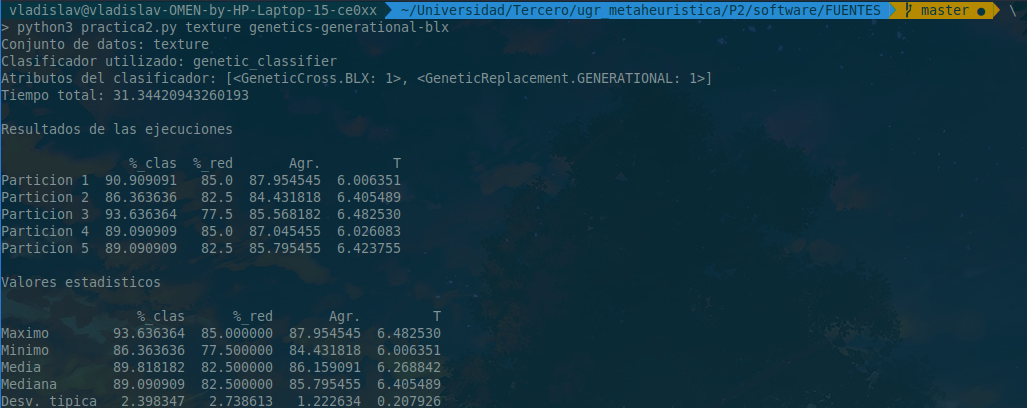
\includegraphics[scale=0.4]{img/out_example.png}
\caption{Ejemplo de salida de la ejecución con los datos \textbf{texture} y el \textbf{AGG}
con operador de cruce BLX-$\alpha$.}
\end{figure}

\newpage

\section{Análisis de resultados y experimentación}

\subsection{Descripción de los casos del problema}

Para analizar el rendimiento de los algoritmos, se han realizado pruebas sobre 3 conjuntos de datos:

\begin{itemize}[label=\textbullet]
	\item \textbf{Colposcopy}: Conjunto de datos de colposcopias adquirido y anotado por médicos profesionales del Hospital
	Universitario de Caracas. Las imágenes fueron tomadas al azar de las secuencias colposcópicas. 287 ejemplos con 62
	características que deben ser clasificados en 2 clases.
	\item \textbf{Ionosphere}: Conjunto de datos de radar que fueron recogidos por un sistema en \textit{Goose Bay},
	Labrador. 352 ejemplos con 34 características que deben ser clasificados en 2 clases.
	\item \textbf{Texture}: Conjunto de datos de extracciones de imágenes para distinguir entre 11 texturas diferentes
	(césped, piel de becerro prensada, papel hecho a mano, rafia en bucle a una pila alta, lienzo de algodón,...). 550
	ejemplos con 40 características que deben ser clasificados en 11 clases.
\end{itemize}

\subsection{Análisis de los resultados}

Se han realizado distintas ejecuciones con los datos para cada uno de los algoritmos. Cada conjunto de datos se ha dividido
con una función de \textbf{sklearn}, y se han mezclado con la \textbf{semialla aleatoria} 40. Antes de ejecutar cada uno de los
algoritmos con la primera partición de datos se ha fijado como \textbf{semilla} el valor 8912374 (la misma que la práctica 
anterior para realizar un análisis más justo, ya que si no podría pasar que alguno de los nuevos algoritmos es mejor). Ambas 
están fijadas en el código y se pueden comprobar. Es muy importante destacar que todas las gráficas que se vean proceden de
la primera partición de cada conjunto de datos, con el objetivo de el análisis sea sobre los mismos datos, en vez de sobre
diferentes particiones.

A continuación se muestran los resultados obtenidos para cada algoritmo y para cada uno de los conjuntos de datos, rescatando
las tablas de la práctica anterior. Se han medido los valores de tasa de clasificación, tasa de reducción, agrupación (función
objetivo) y tiempo que ha tardado (en segundos). Además se ofrece información extra sobre los valores máximo, mínimo, medio,
mediana y desviación típica de cada uno de los datos, para poder comparar los datos más fácilmente. Y, como extra, se ha añadido
una tabla en la que aparecen los valores medios de cada algoritmo, para facilitar la comparación. Estas tablas se pueden ver
a continuación:

\begin{table}[H]
\resizebox{\columnwidth}{!}{%
\begin{tabular}{c|c|c|c|c|c|c|c|c|c|c|c|c|}
\cline{2-13}
\multicolumn{1}{l|}{}                       & \multicolumn{4}{c|}{\textbf{Colposcopy}}                                                   & \multicolumn{4}{c|}{\textbf{Ionosphere}}                                                   & \multicolumn{4}{c|}{\textbf{Texture}}                                                      \\ \cline{2-13} 
\multicolumn{1}{l|}{}                       & \textit{\textbf{\%\_clas}} & \textit{\textbf{\%red}} & \textit{\textbf{Agr.}} & \textbf{T} & \textit{\textbf{\%\_clas}} & \textit{\textbf{\%red}} & \textit{\textbf{Agr.}} & \textbf{T} & \textit{\textbf{\%\_clas}} & \textit{\textbf{\%red}} & \textit{\textbf{Agr.}} & \textbf{T} \\ \hline
\multicolumn{1}{|c|}{\textbf{Partición 1}}  & 79,66                      & 0                       & 39,83                  & 0,00049    & 85,92                      & 0                       & 42,96                  & 0,00045    & 91,82                      & 0                       & 45,91                  & 0,00056    \\ \hline
\multicolumn{1}{|c|}{\textbf{Partición 2}}  & 66,67                      & 0                       & 33,33                  & 0,00037    & 85,71                      & 0                       & 42,86                  & 0,00037    & 91,82                      & 0                       & 45,91                  & 0,00048    \\ \hline
\multicolumn{1}{|c|}{\textbf{Partición 3}}  & 71,93                      & 0                       & 35,96                  & 0,00035    & 88,57                      & 0                       & 44,29                  & 0,00036    & 93,64                      & 0                       & 46,82                  & 0,00044    \\ \hline
\multicolumn{1}{|c|}{\textbf{Partición 4}}  & 82,46                      & 0                       & 41,23                  & 0,00035    & 87,14                      & 0                       & 43,57                  & 0,00039    & 93,64                      & 0                       & 46,82                  & 0,00046    \\ \hline
\multicolumn{1}{|c|}{\textbf{Partición 5}}  & 73,68                      & 0                       & 36,84                  & 0,00035    & 84,29                      & 0                       & 42,14                  & 0,00039    & 90,91                      & 0                       & 45,45                  & 0,00049    \\ \hline
\multicolumn{1}{|c|}{\textbf{Media}}        & 74,88                      & 0                       & 37,44                  & 0,00038    & 86,33                      & 0                       & 43,16                  & 0,00039    & 92,36                      & 0                       & 46,18                  & 0,00049    \\ \hline
\multicolumn{1}{|c|}{\textbf{Máximo}}       & 82,46                      & 0                       & 41,23                  & 0,00049    & 88,57                      & 0                       & 44,29                  & 0,00048    & 93,64                      & 0                       & 46,82                  & 0,00056    \\ \hline
\multicolumn{1}{|c|}{\textbf{Mínimo}}       & 66,67                      & 0                       & 33,33                  & 0,00035    & 84,29                      & 0                       & 42,14                  & 0,00036    & 90,91                      & 0                       & 45,45                  & 0,00044    \\ \hline
\multicolumn{1}{|c|}{\textbf{Mediana}}      & 73,68                      & 0                       & 36,84                  & 0,00035    & 85,92                      & 0                       & 42,96                  & 0,00039    & 91,82                      & 0                       & 45,91                  & 0,00048    \\ \hline
\multicolumn{1}{|c|}{\textbf{Desv. Típica}} & 5,62                       & 0                       & 2,81                   & 0,000056   & 1,44                       & 0                       & 0,72                   & 0,000033   & 1,09                       & 0                       & 0,55                   & 0,00004    \\ \hline
\end{tabular}
}%
\caption{Resultados obtenidos por el algoritmo 1-NN en el problema del APC.}
\end{table}

\begin{table}[H]
\resizebox{\columnwidth}{!}{%
\begin{tabular}{c|c|c|c|c|c|c|c|c|c|c|c|c|}
\cline{2-13}
\multicolumn{1}{l|}{}                       & \multicolumn{4}{c|}{\textbf{Colposcopy}}                                                   & \multicolumn{4}{c|}{\textbf{Ionosphere}}                                                   & \multicolumn{4}{c|}{\textbf{Texture}}                                                      \\ \cline{2-13} 
\multicolumn{1}{l|}{}                       & \textit{\textbf{\%\_clas}} & \textit{\textbf{\%red}} & \textit{\textbf{Agr.}} & \textbf{T} & \textit{\textbf{\%\_clas}} & \textit{\textbf{\%red}} & \textit{\textbf{Agr.}} & \textbf{T} & \textit{\textbf{\%\_clas}} & \textit{\textbf{\%red}} & \textit{\textbf{Agr.}} & \textbf{T} \\ \hline
\multicolumn{1}{|c|}{\textbf{Partición 1}}  & 72,88                      & 29,03                   & 50,96                  & 0,04223180 & 87,32                      & 2,94                    & 45,13                  & 0,04617286 & 93,64                      & 7,50                    & 50,57                  & 0,09011912 \\ \hline
\multicolumn{1}{|c|}{\textbf{Partición 2}}  & 70,18                      & 25,81                   & 47,99                  & 0,03592849 & 91,43                      & 2,94                    & 47,18                  & 0,04701781 & 94,55                      & 15,00                   & 54,77                  & 0,08130646 \\ \hline
\multicolumn{1}{|c|}{\textbf{Partición 3}}  & 68,42                      & 48,39                   & 58,40                  & 0,03983450 & 91,43                      & 2,94                    & 47,18                  & 0,03659153 & 95,45                      & 7,50                    & 51,48                  & 0,08078218 \\ \hline
\multicolumn{1}{|c|}{\textbf{Partición 4}}  & 77,19                      & 64,52                   & 70,85                  & 0,03201556 & 90,00                      & 2,94                    & 46,47                  & 0,03484225 & 97,27                      & 5,00                    & 51,14                  & 0,08749294 \\ \hline
\multicolumn{1}{|c|}{\textbf{Partición 5}}  & 82,46                      & 29,03                   & 55,74                  & 0,03293490 & 84,29                      & 2,94                    & 43,61                  & 0,03472829 & 93,64                      & 2,50                    & 48,07                  & 0,09723902 \\ \hline
\multicolumn{1}{|c|}{\textbf{Media}}        & 74,23                      & 39,35                   & 56,79                  & 0,03658905 & 88,89                      & 2,94                    & 45,92                  & 0,03987055 & 94,91                      & 7,50                    & 51,20                  & 0,08738794 \\ \hline
\multicolumn{1}{|c|}{\textbf{Máximo}}       & 82,46                      & 64,52                   & 70,85                  & 0,04223180 & 91,43                      & 2,94                    & 47,18                  & 0,04701781 & 97,27                      & 15,00                   & 54,77                  & 0,09723902 \\ \hline
\multicolumn{1}{|c|}{\textbf{Mínimo}}       & 68,42                      & 25,81                   & 47,99                  & 0,03201556 & 84,29                      & 2,94                    & 43,61                  & 0,03472829 & 93,64                      & 2,50                    & 48,07                  & 0,08078218 \\ \hline
\multicolumn{1}{|c|}{\textbf{Mediana}}      & 72,88                      & 29,03                   & 55,74                  & 0,03592849 & 90,00                      & 2,94                    & 46,47                  & 0,03659153 & 94,55                      & 7,50                    & 51,14                  & 0,08749294 \\ \hline
\multicolumn{1}{|c|}{\textbf{Desv. Típica}} & 5,07                       & 14,91                   & 7,91                   & 0,00392631 & 2,75                       & 0,00                    & 1,37                   & 0,00553680 & 1,36                       & 4,18                    & 2,15                   & 0,00608498 \\ \hline
\end{tabular}
}%
\caption{Resultados obtenidos por el algoritmo \textit{RELIEF} en el problema del APC.}
\end{table}

\begin{table}[H]
\resizebox{\columnwidth}{!}{%
\begin{tabular}{c|c|c|c|c|c|c|c|c|c|c|c|c|}
\cline{2-13}
                                            & \multicolumn{4}{c|}{\textbf{Colposcopy}}                                                   & \multicolumn{4}{c|}{\textbf{Ionosphere}}                                                   & \multicolumn{4}{c|}{\textbf{Texture}}                                                      \\ \cline{2-13} 
                                            & \textit{\textbf{\%\_clas}} & \textit{\textbf{\%red}} & \textit{\textbf{Agr.}} & \textbf{T} & \textit{\textbf{\%\_clas}} & \textit{\textbf{\%red}} & \textit{\textbf{Agr.}} & \textbf{T} & \textit{\textbf{\%\_clas}} & \textit{\textbf{\%red}} & \textit{\textbf{Agr.}} & \textbf{T} \\ \hline
\multicolumn{1}{|c|}{\textbf{Partición 1}}  & 81,36                      & 83,87                   & 82,61                  & 2,47677159 & 88,73                      & 85,29                   & 87,01                  & 0,74606109 & 92,73                      & 77,50                   & 85,11                  & 0,81571221 \\ \hline
\multicolumn{1}{|c|}{\textbf{Partición 2}}  & 71,93                      & 82,26                   & 77,09                  & 2,88534594 & 88,57                      & 79,41                   & 83,99                  & 0,83731246 & 89,09                      & 85,00                   & 87,05                  & 0,86508775 \\ \hline
\multicolumn{1}{|c|}{\textbf{Partición 3}}  & 70,18                      & 82,26                   & 76,22                  & 2,59485793 & 80,00                      & 94,12                   & 87,06                  & 0,42965746 & 95,45                      & 82,50                   & 88,98                  & 1,02096820 \\ \hline
\multicolumn{1}{|c|}{\textbf{Partición 4}}  & 71,93                      & 82,26                   & 77,09                  & 2,90626860 & 88,57                      & 91,18                   & 89,87                  & 0,75856829 & 90,91                      & 85,00                   & 87,95                  & 1,56289935 \\ \hline
\multicolumn{1}{|c|}{\textbf{Partición 5}}  & 64,91                      & 75,81                   & 70,36                  & 2,81053543 & 85,71                      & 91,18                   & 88,45                  & 0,62555575 & 87,27                      & 82,50                   & 84,89                  & 1,22837043 \\ \hline
\multicolumn{1}{|c|}{\textbf{Media}}        & 72,06                      & 81,29                   & 76,68                  & 2,73475590 & 86,32                      & 88,24                   & 87,28                  & 0,67943101 & 91,09                      & 82,50                   & 86,80                  & 1,09860759 \\ \hline
\multicolumn{1}{|c|}{\textbf{Máximo}}       & 81,36                      & 83,87                   & 82,61                  & 2,90626860 & 88,73                      & 94,12                   & 89,87                  & 0,83731246 & 95,45                      & 85,00                   & 88,98                  & 1,56289935 \\ \hline
\multicolumn{1}{|c|}{\textbf{Mínimo}}       & 64,91                      & 75,81                   & 70,36                  & 2,47677159 & 80,00                      & 79,41                   & 83,99                  & 0,42965746 & 87,27                      & 77,50                   & 84,89                  & 0,81571221 \\ \hline
\multicolumn{1}{|c|}{\textbf{Mediana}}      & 71,93                      & 82,26                   & 77,09                  & 2,81053543 & 88,57                      & 91,18                   & 87,06                  & 0,74606109 & 90,91                      & 82,50                   & 87,05                  & 1,02096820 \\ \hline
\multicolumn{1}{|c|}{\textbf{Desv. Típica}} & 5,31                       & 2,81                    & 3,89                   & 0,16968432 & 3,35                       & 5,26                    & 1,95                   & 0,14206914 & 2,84                       & 2,74                    & 1,59                   & 0,27312796 \\ \hline
\end{tabular}
}%
\caption{Resultados obtenidos por el algoritmo BL en el problema del APC.}
\end{table}

\begin{table}[H]
\resizebox{\columnwidth}{!}{%
\begin{tabular}{c|c|c|c|c|c|c|c|c|c|c|c|c|}
\cline{2-13}
                                            & \multicolumn{4}{c|}{\textbf{Colposcopy}}                                 & \multicolumn{4}{c|}{\textbf{Ionosphere}}                        & \multicolumn{4}{c|}{\textbf{Texture}}                           \\ \cline{2-13} 
                                            & \textit{\textbf{\%\_clas}} & \textit{\textbf{\%red}} & \textit{\textbf{Agr.}} & \textbf{T} & \textit{\textbf{\%\_clas}} & \textit{\textbf{\%red}} & \textit{\textbf{Agr.}} & \textbf{T} & \textit{\textbf{\%\_clas}} & \textit{\textbf{\%red}} & \textit{\textbf{Agr.}} & \textbf{T} \\ \hline
\multicolumn{1}{|c|}{\textbf{Partición 1}}  & 77.97             & 72.58                   & 75.27         & 10.26      & 83.1              & 85.29          & 84.2          & 5.0        & 90.91             & 85.0           & 87.95         & 6.29       \\ \hline
\multicolumn{1}{|c|}{\textbf{Partición 2}}  & 66.67             & 72.58                   & 69.62         & 10.79      & 82.86             & 88.24          & 85.55         & 4.36       & 86.36             & 82.5           & 84.43         & 6.63       \\ \hline
\multicolumn{1}{|c|}{\textbf{Partición 3}}  & 78.95             & 59.68                   & 69.31         & 13.95      & 88.57             & 85.29          & 86.93         & 4.69       & 93.64             & 77.5           & 85.57         & 6.88       \\ \hline
\multicolumn{1}{|c|}{\textbf{Partición 4}}  & 77.19             & 74.19                   & 75.69         & 9.55       & 91.43             & 91.18          & 91.3          & 3.88       & 89.09             & 85.0           & 87.05         & 6.26       \\ \hline
\multicolumn{1}{|c|}{\textbf{Partición 5}}  & 71.93             & 72.58                   & 72.26         & 10.97      & 81.43             & 76.47          & 78.95         & 5.98       & 89.09             & 82.5           & 85.8          & 6.28       \\ \hline
\multicolumn{1}{|c|}{\textbf{Media}}        & 74.54             & 70.32                   & 72.43         & 11.1       & 85.48             & 85.29          & 85.39         & 4.78       & 89.82             & 82.5           & 86.16         & 6.47       \\ \hline
\multicolumn{1}{|c|}{\textbf{Máximo}}       & 78.95             & 74.19                   & 75.69         & 13.95      & 91.43             & 91.18          & 91.3          & 5.98       & 93.64             & 85.0           & 87.95         & 6.88       \\ \hline
\multicolumn{1}{|c|}{\textbf{Mínimo}}       & 66.67             & 59.68                   & 69.31         & 9.55       & 81.43             & 76.47          & 78.95         & 3.88       & 86.36             & 77.5           & 84.43         & 6.26       \\ \hline
\multicolumn{1}{|c|}{\textbf{Mediana}}      & 77.19             & 72.58                   & 72.26         & 10.79      & 83.1              & 85.29          & 85.55         & 4.69       & 89.09             & 82.5           & 85.8          & 6.29       \\ \hline
\multicolumn{1}{|c|}{\textbf{Desv. Típica}} & 4.63              & 5.36                    & 2.7           & 1.51       & 3.84              & 4.92           & 4.01          & 0.7        & 2.4               & 2.74           & 1.22          & 0.25       \\ \hline
\end{tabular}
}%
\caption{Resultados obtenidos por el AGG con cruce BLX-$\alpha$ en el problema del APC.}
\end{table}

\begin{table}[H]
\resizebox{\columnwidth}{!}{%
\begin{tabular}{c|c|c|c|c|c|c|c|c|c|c|c|c|}
\cline{2-13}
                                            & \multicolumn{4}{c|}{\textbf{Colposcopy}}                                 & \multicolumn{4}{c|}{\textbf{Ionosphere}}                        & \multicolumn{4}{c|}{\textbf{Texture}}                           \\ \cline{2-13} 
                                            & \textit{\textbf{\%\_clas}} & \textit{\textbf{\%red}} & \textit{\textbf{Agr.}} & \textbf{T} & \textit{\textbf{\%\_clas}} & \textit{\textbf{\%red}} & \textit{\textbf{Agr.}} & \textbf{T} & \textit{\textbf{\%\_clas}} & \textit{\textbf{\%red}} & \textit{\textbf{Agr.}} & \textbf{T} \\ \hline
\multicolumn{1}{|c|}{\textbf{Partición 1}}  & 81.36             & 58.06                   & 69.71         & 18.7       & 87.32             & 61.76          & 74.54         & 9.83       & 93.64             & 75.0           & 84.32         & 8.72       \\ \hline
\multicolumn{1}{|c|}{\textbf{Partición 2}}  & 73.68             & 51.61                   & 62.65         & 17.91      & 85.71             & 70.59          & 78.15         & 9.98       & 90.91             & 77.5           & 84.2          & 8.04       \\ \hline
\multicolumn{1}{|c|}{\textbf{Partición 3}}  & 66.67             & 54.84                   & 60.75         & 14.76      & 90.0              & 64.71          & 77.35         & 9.03       & 92.73             & 62.5           & 77.61         & 10.16      \\ \hline
\multicolumn{1}{|c|}{\textbf{Partición 4}}  & 78.95             & 54.84                   & 66.89         & 16.96      & 91.43             & 64.71          & 78.07         & 8.22       & 90.91             & 67.5           & 79.2          & 9.85       \\ \hline
\multicolumn{1}{|c|}{\textbf{Partición 5}}  & 71.93             & 48.39                   & 60.16         & 18.4       & 81.43             & 61.76          & 71.6          & 10.36      & 90.91             & 55.0           & 72.95         & 12.62      \\ \hline
\multicolumn{1}{|c|}{\textbf{Media}}        & 74.52             & 53.55                   & 64.03         & 17.35      & 87.18             & 64.71          & 75.94         & 9.48       & 91.82             & 67.5           & 79.66         & 9.88       \\ \hline
\multicolumn{1}{|c|}{\textbf{Máximo}}       & 81.36             & 58.06                   & 69.71         & 18.7       & 91.43             & 70.59          & 78.15         & 10.36      & 93.64             & 77.5           & 84.32         & 12.62      \\ \hline
\multicolumn{1}{|c|}{\textbf{Mínimo}}       & 66.67             & 48.39                   & 60.16         & 14.76      & 81.43             & 61.76          & 71.6          & 8.22       & 90.91             & 55.0           & 72.95         & 8.04       \\ \hline
\multicolumn{1}{|c|}{\textbf{Mediana}}      & 73.68             & 54.84                   & 62.65         & 17.91      & 87.32             & 64.71          & 77.35         & 9.83       & 90.91             & 67.5           & 79.2          & 9.85       \\ \hline
\multicolumn{1}{|c|}{\textbf{Desv. Típica}} & 5.2               & 3.29                    & 3.69          & 1.42       & 3.5               & 3.22           & 2.54          & 0.76       & 1.15              & 8.22           & 4.28          & 1.57       \\ \hline
\end{tabular}
}%
\caption{Resultados obtenidos por el AGG con cruce aritmético en el problema del APC.}
\end{table}


\begin{table}[H]
\resizebox{\columnwidth}{!}{%
\begin{tabular}{c|c|c|c|c|c|c|c|c|c|c|c|c|}
\cline{2-13}
                                            & \multicolumn{4}{c|}{\textbf{Colposcopy}}                                 & \multicolumn{4}{c|}{\textbf{Ionosphere}}                        & \multicolumn{4}{c|}{\textbf{Texture}}                           \\ \cline{2-13} 
                                            & \textit{\textbf{\%\_clas}} & \textit{\textbf{\%red}} & \textit{\textbf{Agr.}} & \textbf{T} & \textit{\textbf{\%\_clas}} & \textit{\textbf{\%red}} & \textit{\textbf{Agr.}} & \textbf{T} & \textit{\textbf{\%\_clas}} & \textit{\textbf{\%red}} & \textit{\textbf{Agr.}} & \textbf{T} \\ \hline
\multicolumn{1}{|c|}{\textbf{Partición 1}}  & 69.49             & 72.58                   & 71.04         & 11.01      & 88.73             & 91.18          & 89.95         & 5.58       & 88.18             & 80.0           & 84.09         & 8.03       \\ \hline
\multicolumn{1}{|c|}{\textbf{Partición 2}}  & 71.93             & 70.97                   & 71.45         & 11.7       & 85.71             & 88.24          & 86.97         & 6.71       & 85.45             & 75.0           & 80.23         & 7.94       \\ \hline
\multicolumn{1}{|c|}{\textbf{Partición 3}}  & 68.42             & 64.52                   & 66.47         & 13.99      & 81.43             & 82.35          & 81.89         & 8.23       & 94.55             & 85.0           & 89.77         & 6.83       \\ \hline
\multicolumn{1}{|c|}{\textbf{Partición 4}}  & 77.19             & 80.65                   & 78.92         & 10.92      & 80.0              & 85.29          & 82.65         & 5.73       & 94.55             & 67.5           & 81.02         & 10.15      \\ \hline
\multicolumn{1}{|c|}{\textbf{Partición 5}}  & 71.93             & 70.97                   & 71.45         & 11.41      & 84.29             & 79.41          & 81.85         & 6.69       & 91.82             & 77.5           & 84.66         & 8.06       \\ \hline
\multicolumn{1}{|c|}{\textbf{Media}}        & 71.79             & 71.94                   & 71.86         & 11.81      & 84.03             & 85.29          & 84.66         & 6.59       & 90.91             & 77.0           & 83.95         & 8.2        \\ \hline
\multicolumn{1}{|c|}{\textbf{Máximo}}       & 77.19             & 80.65                   & 78.92         & 13.99      & 88.73             & 91.18          & 89.95         & 8.23       & 94.55             & 85.0           & 89.77         & 10.15      \\ \hline
\multicolumn{1}{|c|}{\textbf{Mínimo}}       & 68.42             & 64.52                   & 66.47         & 10.92      & 80.0              & 79.41          & 81.85         & 5.58       & 85.45             & 67.5           & 80.23         & 6.83       \\ \hline
\multicolumn{1}{|c|}{\textbf{Mediana}}      & 71.93             & 70.97                   & 71.45         & 11.41      & 84.29             & 85.29          & 82.65         & 6.69       & 91.82             & 77.5           & 84.09         & 8.03       \\ \hline
\multicolumn{1}{|c|}{\textbf{Desv. Típica}} & 3.03              & 5.16                    & 4.0           & 1.13       & 3.1               & 4.16           & 3.26          & 0.94       & 3.59              & 5.79           & 3.37          & 1.07       \\ \hline
\end{tabular}
}%
\caption{Resultados obtenidos por el AGE con cruce BLX-$\alpha$ en el problema del APC.}
\end{table}

\begin{table}[H]
\resizebox{\columnwidth}{!}{%
\begin{tabular}{c|c|c|c|c|c|c|c|c|c|c|c|c|}
\cline{2-13}
                                            & \multicolumn{4}{c|}{\textbf{Colposcopy}}                                 & \multicolumn{4}{c|}{\textbf{Ionosphere}}                        & \multicolumn{4}{c|}{\textbf{Texture}}                           \\ \cline{2-13} 
                                            & \textit{\textbf{\%\_clas}} & \textit{\textbf{\%red}} & \textit{\textbf{Agr.}} & \textbf{T} & \textit{\textbf{\%\_clas}} & \textit{\textbf{\%red}} & \textit{\textbf{Agr.}} & \textbf{T} & \textit{\textbf{\%\_clas}} & \textit{\textbf{\%red}} & \textit{\textbf{Agr.}} & \textbf{T} \\ \hline
\multicolumn{1}{|c|}{\textbf{Partición 1}}  & 74.58             & 59.68                   & 67.13         & 15.52      & 85.92             & 61.76          & 73.84         & 10.09      & 95.45             & 72.5           & 83.98         & 9.33       \\ \hline
\multicolumn{1}{|c|}{\textbf{Partición 2}}  & 68.42             & 66.13                   & 67.28         & 13.6       & 87.14             & 64.71          & 75.92         & 11.17      & 90.0              & 75.0           & 82.5          & 9.81       \\ \hline
\multicolumn{1}{|c|}{\textbf{Partición 3}}  & 68.42             & 67.74                   & 68.08         & 14.62      & 90.0              & 73.53          & 81.76         & 8.93       & 89.09             & 70.0           & 79.55         & 9.6        \\ \hline
\multicolumn{1}{|c|}{\textbf{Partición 4}}  & 77.19             & 69.35                   & 73.27         & 12.62      & 85.71             & 64.71          & 75.21         & 11.07      & 82.73             & 70.0           & 76.36         & 10.9       \\ \hline
\multicolumn{1}{|c|}{\textbf{Partición 5}}  & 70.18             & 69.35                   & 69.77         & 11.34      & 84.29             & 70.59          & 77.44         & 11.03      & 91.82             & 72.5           & 82.16         & 10.52      \\ \hline
\multicolumn{1}{|c|}{\textbf{Media}}        & 71.76             & 66.45                   & 69.1          & 13.54      & 86.61             & 67.06          & 76.84         & 10.46      & 89.82             & 72.0           & 80.91         & 10.03      \\ \hline
\multicolumn{1}{|c|}{\textbf{Máximo}}       & 77.19             & 69.35                   & 73.27         & 15.52      & 90.0              & 73.53          & 81.76         & 11.17      & 95.45             & 75.0           & 83.98         & 10.9       \\ \hline
\multicolumn{1}{|c|}{\textbf{Mínimo}}       & 68.42             & 59.68                   & 67.13         & 11.34      & 84.29             & 61.76          & 73.84         & 8.93       & 82.73             & 70.0           & 76.36         & 9.33       \\ \hline
\multicolumn{1}{|c|}{\textbf{Mediana}}      & 70.18             & 67.74                   & 68.08         & 13.6       & 85.92             & 64.71          & 75.92         & 11.03      & 90.0              & 72.5           & 82.16         & 9.81       \\ \hline
\multicolumn{1}{|c|}{\textbf{Desv. Típica}} & 3.53              & 3.59                    & 2.29          & 1.47       & 1.92              & 4.32           & 2.72          & 0.86       & 4.16              & 1.87           & 2.68          & 0.59       \\ \hline
\end{tabular}
}%
\caption{Resultados obtenidos por el AGE con cruce aritmético en el problema del APC.}
\end{table}

\begin{table}[H]
\resizebox{\columnwidth}{!}{%
\begin{tabular}{c|c|c|c|c|c|c|c|c|c|c|c|c|}
\cline{2-13}
                                            & \multicolumn{4}{c|}{\textbf{Colposcopy}}                                 & \multicolumn{4}{c|}{\textbf{Ionosphere}}                        & \multicolumn{4}{c|}{\textbf{Texture}}                           \\ \cline{2-13} 
                                            & \textit{\textbf{\%\_clas}} & \textit{\textbf{\%red}} & \textit{\textbf{Agr.}} & \textbf{T} & \textit{\textbf{\%\_clas}} & \textit{\textbf{\%red}} & \textit{\textbf{Agr.}} & \textbf{T} & \textit{\textbf{\%\_clas}} & \textit{\textbf{\%red}} & \textit{\textbf{Agr.}} & \textbf{T} \\ \hline
\multicolumn{1}{|c|}{\textbf{Partición 1}}  & 69.49             & 85.48                   & 77.49         & 7.15       & 80.28             & 88.24          & 84.26         & 3.91       & 88.18             & 85.0           & 86.59         & 4.74       \\ \hline
\multicolumn{1}{|c|}{\textbf{Partición 2}}  & 68.42             & 80.65                   & 74.53         & 8.19       & 87.14             & 88.24          & 87.69         & 3.57       & 87.27             & 85.0           & 86.14         & 5.23       \\ \hline
\multicolumn{1}{|c|}{\textbf{Partición 3}}  & 80.7              & 83.87                   & 82.29         & 7.56       & 75.71             & 88.24          & 81.97         & 3.82       & 93.64             & 82.5           & 88.07         & 5.51       \\ \hline
\multicolumn{1}{|c|}{\textbf{Partición 4}}  & 84.21             & 83.87                   & 84.04         & 7.8        & 85.71             & 94.12          & 89.92         & 3.43       & 91.82             & 85.0           & 88.41         & 5.39       \\ \hline
\multicolumn{1}{|c|}{\textbf{Partición 5}}  & 78.95             & 83.87                   & 81.41         & 7.79       & 84.29             & 91.18          & 87.73         & 3.68       & 92.73             & 82.5           & 87.61         & 5.75       \\ \hline
\multicolumn{1}{|c|}{\textbf{Media}}        & 76.35             & 83.55                   & 79.95         & 7.7        & 82.63             & 90.0           & 86.31         & 3.68       & 90.73             & 84.0           & 87.36         & 5.32       \\ \hline
\multicolumn{1}{|c|}{\textbf{Máximo}}       & 84.21             & 85.48                   & 84.04         & 8.19       & 87.14             & 94.12          & 89.92         & 3.91       & 93.64             & 85.0           & 88.41         & 5.75       \\ \hline
\multicolumn{1}{|c|}{\textbf{Mínimo}}       & 68.42             & 80.65                   & 74.53         & 7.15       & 75.71             & 88.24          & 81.97         & 3.43       & 87.27             & 82.5           & 86.14         & 4.74       \\ \hline
\multicolumn{1}{|c|}{\textbf{Mediana}}      & 78.95             & 83.87                   & 81.41         & 7.79       & 84.29             & 88.24          & 87.69         & 3.68       & 91.82             & 85.0           & 87.61         & 5.39       \\ \hline
\multicolumn{1}{|c|}{\textbf{Desv. Típica}} & 6.28              & 1.58                    & 3.46          & 0.34       & 4.15              & 2.35           & 2.83          & 0.17       & 2.53              & 1.22           & 0.87          & 0.34       \\ \hline
\end{tabular}
}%
\caption{Resultados obtenidos por el AM con cruce BLX-$\alpha$ y Búsqueda Local sobre toda la población en el problema del
APC.}
\end{table}

\begin{table}[H]
\resizebox{\columnwidth}{!}{%
\begin{tabular}{c|c|c|c|c|c|c|c|c|c|c|c|c|}
\cline{2-13}
                                            & \multicolumn{4}{c|}{\textbf{Colposcopy}}                                 & \multicolumn{4}{c|}{\textbf{Ionosphere}}                        & \multicolumn{4}{c|}{\textbf{Texture}}                           \\ \cline{2-13} 
                                            & \textit{\textbf{\%\_clas}} & \textit{\textbf{\%red}} & \textit{\textbf{Agr.}} & \textbf{T} & \textit{\textbf{\%\_clas}} & \textit{\textbf{\%red}} & \textit{\textbf{Agr.}} & \textbf{T} & \textit{\textbf{\%\_clas}} & \textit{\textbf{\%red}} & \textit{\textbf{Agr.}} & \textbf{T} \\ \hline
\multicolumn{1}{|c|}{\textbf{Partición 1}}  & 72.88             & 83.87                   & 78.38         & 5.88       & 90.14             & 91.18          & 90.66         & 2.94       & 87.27             & 85.0           & 86.14         & 4.31       \\ \hline
\multicolumn{1}{|c|}{\textbf{Partición 2}}  & 71.93             & 83.87                   & 77.9          & 6.73       & 90.0              & 91.18          & 90.59         & 2.97       & 90.91             & 87.5           & 89.2          & 4.22       \\ \hline
\multicolumn{1}{|c|}{\textbf{Partición 3}}  & 70.18             & 83.87                   & 77.02         & 6.62       & 94.29             & 82.35          & 88.32         & 3.85       & 95.45             & 87.5           & 91.48         & 4.35       \\ \hline
\multicolumn{1}{|c|}{\textbf{Partición 4}}  & 75.44             & 80.65                   & 78.04         & 8.95       & 90.0              & 82.35          & 86.18         & 4.7        & 85.45             & 87.5           & 86.48         & 4.48       \\ \hline
\multicolumn{1}{|c|}{\textbf{Partición 5}}  & 59.65             & 82.26                   & 70.95         & 7.66       & 87.14             & 91.18          & 89.16         & 2.75       & 81.82             & 85.0           & 83.41         & 4.58       \\ \hline
\multicolumn{1}{|c|}{\textbf{Media}}        & 70.01             & 82.9                    & 76.46         & 7.17       & 90.31             & 87.65          & 88.98         & 3.44       & 88.18             & 86.5           & 87.34         & 4.39       \\ \hline
\multicolumn{1}{|c|}{\textbf{Máximo}}       & 75.44             & 83.87                   & 78.38         & 8.95       & 94.29             & 91.18          & 90.66         & 4.7        & 95.45             & 87.5           & 91.48         & 4.58       \\ \hline
\multicolumn{1}{|c|}{\textbf{Mínimo}}       & 59.65             & 80.65                   & 70.95         & 5.88       & 87.14             & 82.35          & 86.18         & 2.75       & 81.82             & 85.0           & 83.41         & 4.22       \\ \hline
\multicolumn{1}{|c|}{\textbf{Mediana}}      & 71.93             & 83.87                   & 77.9          & 6.73       & 90.0              & 91.18          & 89.16         & 2.97       & 87.27             & 87.5           & 86.48         & 4.35       \\ \hline
\multicolumn{1}{|c|}{\textbf{Desv. Típica}} & 5.45              & 1.29                    & 2.79          & 1.06       & 2.28              & 4.32           & 1.66          & 0.73       & 4.67              & 1.22           & 2.77          & 0.13       \\ \hline
\end{tabular}
}%
\caption{Resultados obtenidos por el AM con cruce BLX-$\alpha$ y Búsqueda Local sobre el mejor de la población en el problema
del APC.}
\end{table}

\begin{table}[H]
\resizebox{\columnwidth}{!}{%
\begin{tabular}{c|c|c|c|c|c|c|c|c|c|c|c|c|}
\cline{2-13}
                                            & \multicolumn{4}{c|}{\textbf{Colposcopy}}                                 & \multicolumn{4}{c|}{\textbf{Ionosphere}}                        & \multicolumn{4}{c|}{\textbf{Texture}}                           \\ \cline{2-13} 
                                            & \textit{\textbf{\%\_clas}} & \textit{\textbf{\%red}} & \textit{\textbf{Agr.}} & \textbf{T} & \textit{\textbf{\%\_clas}} & \textit{\textbf{\%red}} & \textit{\textbf{Agr.}} & \textbf{T} & \textit{\textbf{\%\_clas}} & \textit{\textbf{\%red}} & \textit{\textbf{Agr.}} & \textbf{T} \\ \hline
\multicolumn{1}{|c|}{\textbf{Partición 1}}  & 72.88             & 83.87                   & 78.38         & 5.88       & 90.14             & 91.18          & 90.66         & 2.94       & 87.27             & 85.0           & 86.14         & 4.31       \\ \hline
\multicolumn{1}{|c|}{\textbf{Partición 2}}  & 71.93             & 83.87                   & 77.9          & 6.73       & 90.0              & 91.18          & 90.59         & 2.97       & 90.91             & 87.5           & 89.2          & 4.22       \\ \hline
\multicolumn{1}{|c|}{\textbf{Partición 3}}  & 70.18             & 83.87                   & 77.02         & 6.62       & 94.29             & 82.35          & 88.32         & 3.85       & 95.45             & 87.5           & 91.48         & 4.35       \\ \hline
\multicolumn{1}{|c|}{\textbf{Partición 4}}  & 75.44             & 80.65                   & 78.04         & 8.95       & 90.0              & 82.35          & 86.18         & 4.7        & 85.45             & 87.5           & 86.48         & 4.48       \\ \hline
\multicolumn{1}{|c|}{\textbf{Partición 5}}  & 59.65             & 82.26                   & 70.95         & 7.66       & 87.14             & 91.18          & 89.16         & 2.75       & 81.82             & 85.0           & 83.41         & 4.58       \\ \hline
\multicolumn{1}{|c|}{\textbf{Media}}        & 70.01             & 82.9                    & 76.46         & 7.17       & 90.31             & 87.65          & 88.98         & 3.44       & 88.18             & 86.5           & 87.34         & 4.39       \\ \hline
\multicolumn{1}{|c|}{\textbf{Máximo}}       & 75.44             & 83.87                   & 78.38         & 8.95       & 94.29             & 91.18          & 90.66         & 4.7        & 95.45             & 87.5           & 91.48         & 4.58       \\ \hline
\multicolumn{1}{|c|}{\textbf{Mínimo}}       & 59.65             & 80.65                   & 70.95         & 5.88       & 87.14             & 82.35          & 86.18         & 2.75       & 81.82             & 85.0           & 83.41         & 4.22       \\ \hline
\multicolumn{1}{|c|}{\textbf{Mediana}}      & 71.93             & 83.87                   & 77.9          & 6.73       & 90.0              & 91.18          & 89.16         & 2.97       & 87.27             & 87.5           & 86.48         & 4.35       \\ \hline
\multicolumn{1}{|c|}{\textbf{Desv. Típica}} & 5.45              & 1.29                    & 2.79          & 1.06       & 2.28              & 4.32           & 1.66          & 0.73       & 4.67              & 1.22           & 2.77          & 0.13       \\ \hline
\end{tabular}
}%
\caption{Resultados obtenidos por el AM con cruce BLX-$\alpha$ y Búsqueda Local sobre un cromosoma aleatorio  de la población
en el problema del APC.}
\end{table}

\begin{table}[H]
\resizebox{\columnwidth}{!}{%
\begin{tabular}{c|c|c|c|c|c|c|c|c|c|c|c|c|}
\cline{2-13}
                                              & \multicolumn{4}{c|}{\textbf{Colposcopy}}                                 & \multicolumn{4}{c|}{\textbf{Ionosphere}}                        & \multicolumn{4}{c|}{\textbf{Texture}}                           \\ \cline{2-13} 
                                              & \textit{\textbf{\%\_clas}} & \textit{\textbf{\%red}} & \textit{\textbf{Agr.}} & \textbf{T} & \textit{\textbf{\%\_clas}} & \textit{\textbf{\%red}} & \textit{\textbf{Agr.}} & \textbf{T} & \textit{\textbf{\%\_clas}} & \textit{\textbf{\%red}} & \textit{\textbf{Agr.}} & \textbf{T} \\ \hline
\multicolumn{1}{|c|}{\textbf{1-NN}}           & 74,88             & 0                       & 37,44         & 0.00039    & 86,33             & 0              & 43,16         & 0.00039    & 92,36             & 0              & 46,18         & 0.00049    \\ \hline
\multicolumn{1}{|c|}{\textbf{RELIEF}}         & 74,23             & 39,35                   & 56,79         & 0.03659    & 88,89             & 2,94           & 45,92         & 0.03987    & 94,91             & 7,50           & 51,20         & 0.08739    \\ \hline
\multicolumn{1}{|c|}{\textbf{BL}}             & 72,06             & 81,29                   & 76,68         & 2.73476    & 86,32             & 88,24          & 87,28         & 0.67943    & 91,09             & 82,50          & 86,80         & 1.09861    \\ \hline
\multicolumn{1}{|c|}{\textbf{AGG-BLX}}        & 74.54             & 70.32                   & 72.43         & 11.1       & 85.48             & 85.29          & 85.39         & 4.78       & 89.82             & 82.5           & 86.16         & 6.47       \\ \hline
\multicolumn{1}{|c|}{\textbf{AGG-CA}}         & 74.52             & 53.55                   & 64.03         & 17.35      & 87.18             & 64.71          & 75.94         & 9.48       & 91.82             & 67.5           & 79.66         & 9.88       \\ \hline
\multicolumn{1}{|c|}{\textbf{AGE-BLX}}        & 71.79             & 71.94                   & 71.86         & 11.81      & 84.03             & 85.29          & 84.66         & 6.59       & 90.91             & 77.0           & 83.95         & 8.2        \\ \hline
\multicolumn{1}{|c|}{\textbf{AGE-CA}}         & 71.76             & 66.45                   & 69.1          & 13.54      & 86.61             & 67.06          & 76.84         & 10.46      & 89.82             & 72.0           & 80.91         & 10.03      \\ \hline
\multicolumn{1}{|c|}{\textbf{AM-(10,1.0)}}    & 76.35             & 83.55                   & 79.95         & 7.7        & 82.63             & 90.0           & 86.31         & 3.68       & 90.73             & 84.0           & 87.36         & 5.32       \\ \hline
\multicolumn{1}{|c|}{\textbf{AM-(10,0.1)}}    & 73.87             & 83.23                   & 78.55         & 6.14       & 86.03             & 88.82          & 87.43         & 3.22       & 89.27             & 86.0           & 87.64         & 4.52       \\ \hline
\multicolumn{1}{|c|}{\textbf{AM-(10,0.1mej)}} & 70.01             & 82.9                    & 76.46         & 7.17       & 90.31             & 87.65          & 88.98         & 3.44       & 88.18             & 86.5           & 87.34         & 4.39       \\ \hline
\end{tabular}
}%
\caption{Valores medios de los distintos algoritmos para el problema del APC.}
\end{table}

Antes de realizar el análisis, vamos a describir como se realizará el proceso. Primero se compararán los algoritmos de la misma
categoría (AGG, AGE y AM). Después, se compararán los mejores genéticos para decidir cuál es el mejor. Luego se compararán los AG
con los AM para ver cuál de las dos metaheurísticas tiene un mejor rendimiento. Finalmente se comparará la mejor metaheurística
implementada en esta práctica con los algoritmos de comparación, y se elegirá el mejor. Todo esto se hará para cada conjunto de
datos, y se llegará a una conclusión.

Para realizar la comparación se atenderán los siguientes criterios:

\begin{itemize}
	\item En caso de comparar los AGG, AGE y AM, se mirarán los valores medios de tasa de clasificación, tasa de reducción,
	agrupación y, en menor medida, el tiempo. El mejor de los algoritmos será el que destaque en más campos.
	\item A la hora de comparar la mejor metaheurística de esta práctica con los algoritmos de comparación, si se compara con
	la búsqueda local se mirarán todas las características anterires menos el tiempo. En caso de compararla con alguna
	de las otras, solo se mirará la tasa de clasificación, ya que no sería justo comparar las otras características porque esas
	técnicas no reducen o su objetivo no es reducir ni maximizar un valor \textit{fitness}.
\end{itemize}

Con esto dicho, comencemos el análisis.

Vamos a comenzar por el conjunto de datos \textit{Colposcopy}. Comenzando por los AGG, nos encontramos que el AGG con cruce
BLX-$\alpha$ es muy superior al AGG con cruce aritmético, ya que todos sus valores medios son más elevados que los de su
contraparte. Solo en el caso de la tasa de clasificación tienen valores muy cercanos, debido a que puede ser que se haya
producido \textit{overfitting} con el entrenamiento, pero en el resto de casos, reduce más, tiene una mayor tasa de agrupación y,
de media, tarda menos, lo cuál siempre es un punto fuerte en este tipo de metaheurísticas.

Si echamos un vistazo a los AGE vemos que sucede algo similar, ya que los valores obtenidos por el BLX-$\alpha$ son superiores
en todos los aspectos menos en clasificación, donde a pesar de ser superiores, la diferencia es muy poca (solo de 0.03). Por tanto
ya tenemos un claro mejor AGE de entre los dos.

Observando los AM nos encontramos con que, en este caso, el AM que aplica la búsqueda local sobre toda la población es el mejor.
Hay que tener en cuenta que los AM se han construido sobre el AGG con operador de cruce BLX-$\alpha$ y sobre esta base se ha
introducido una búsqueda local, con lo cuál, los resultados obtenidos se espera que sean o bien muy próximos a los del genético
o bien un poco superiores. Volviendo a nuestra comparación de los AM, el algoritmo que aplica la búsqueda local sobre toda la
población domina a los otros en casi todos los aspectos, ya que produce mejores tasas de clasificación y reducción y una mejor
agrupación, pero en cuanto a tiempo pierde contra el que aplica una búsqueda local sobre un cromosoma aleatorio. El segundo mejor
memético sería el que aplica la búsqueda local sobre un cromosoma aleatorio, y en último lugar iría el que lo hace sobre el
mejor de la población. De aquí podemos pensar que al aplicar la BL sobre el mejor se pueden dar problemas, ya que si los
descendientes que genera el mejor cromosoma son peores que él, no hay nada que se pueda hacer, por mucho elitismo que se tenga.
Puede ser que el mejor se haya optimizado tanto que haya caído en un óptimo local, y que al aplicar sobre él una búsqueda local no
se obtengan unos buenos resultados, y que además, por mucho que se le cruce con otros cromosomas, como son peores que él, no se
produce una mejora real. En conclusión, en este problema el mejor AM es el que aplica la búsqueda local sobre toda la población,
ya que combina una estrategia de explorar con los genéticos y de explotar con la búsqueda local, teniendo distintos cromosomas
en diferentes regiones del espacio con muy buenos valores (aunque también puede pasar que todos estén en la misma zona pero tengan
unos valores \textit{fitness} muy buenos.

Para ver un poco mejor los AM, se han extraído las siguientes gráficas:

\begin{figure}[H]
\centering
\begin{minipage}{.5\textwidth}
	\centering
	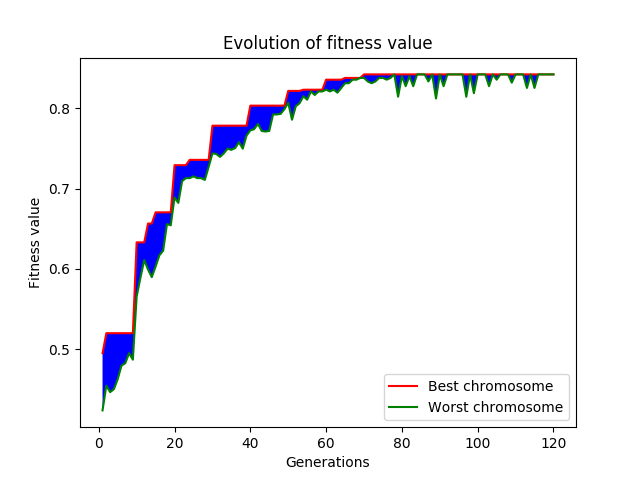
\includegraphics[scale=0.43]{img/am-all-colposcopy.png}
	\caption{Evolución del mejor y peor cromosoma de la población.}
\end{minipage}%
\begin{minipage}{.5\textwidth}
	\centering
	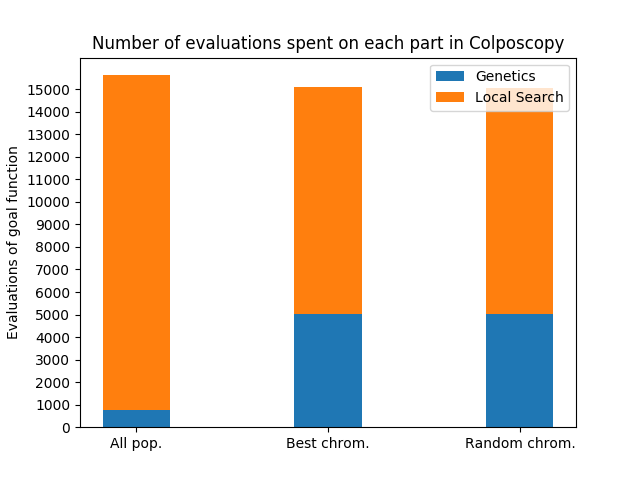
\includegraphics[scale=0.43]{img/bars-colposcopy.png}
	\caption{Comparación entre las evaluaciones en los AM.}
\end{minipage}
\end{figure}

Como se puede ver, los valores \textit{fitness} de la población pegan picos cuando se aplica la búsqueda local sobre ellos y
suben mucho, excepto casi al final, donde se estancan y van subiendo y bajando en el caso del peor cromosoma, probablemente
debido a los cruces o a que una mutación ha hecho que baje el \textit{fitness}. En el segundo gráfico se puede ver como
la búsqueda local representa un mayor número de evaluaciones en caso de aplicarla sobre toda la población que la parte de los
genéticos, mientras que en los otros dos casos los números son muy similares, ya que aplicarlo sobre un cromosoma aleatorio
o el mejor conducirá a realizar aproximadamente el mismo número de evaluaciones en cada parte. Por tanto, al aplicar la BL
sobre toda la población se está explotando más de lo que se explora, lo cuál puede llevar a malos resultados en otros problemas.

Volviendo a los genéticos, nos encontramos que el mejor de ellos es el AGG con BLX, ya que supera a su contraparte de los AGE
en casi todos los aspectos menos en reducción media, donde se ve un poco reducido respecto a su homónimo. Por tanto, el mejor
de los 2 es el AGG con BLX.

En las siguientes gráficas se puede ver un poco el funcionamiento de los distintos genéticos:

\begin{figure}[H]
\centering
\begin{minipage}{.5\textwidth}
	\centering
	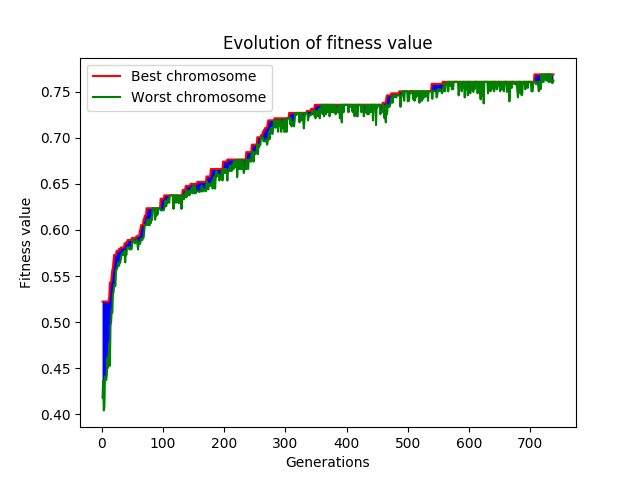
\includegraphics[scale=0.43]{img/agg-blx-colposcopy.png}
	\caption{AGG con BLX.}
\end{minipage}%
\begin{minipage}{.5\textwidth}
	\centering
	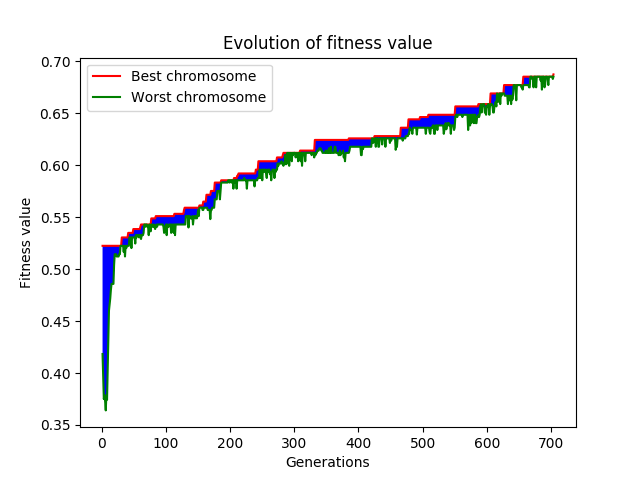
\includegraphics[scale=0.43]{img/agg-ac-colposcopy.png}
	\caption{AGG con cruce aritmético.}
\end{minipage}
\end{figure}

\begin{figure}[H]
\centering
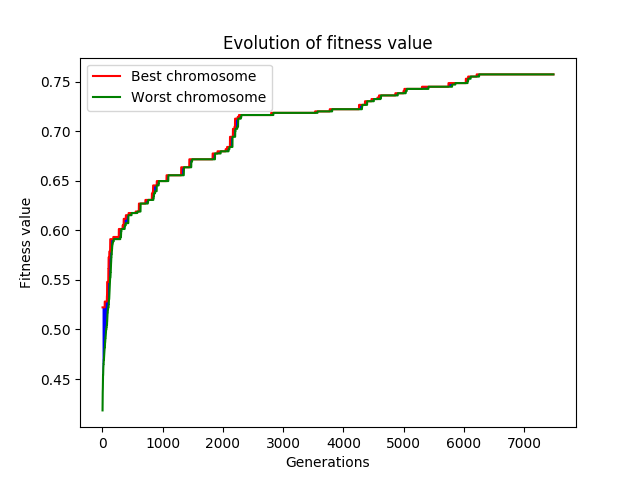
\includegraphics[scale=0.6]{img/age-blx-colposcopy.png}
\caption{AGE con BLX.}
\end{figure}

Como se puede ver, el AGG con BLX crece más partiendo de un valor muy similar a los otros, y se estanca menos veces, aunque a
partir de las 300 generaciones crece muy poco a poco, ya que los resultados van convergiendo. En el caso del AGG con CA sucede
algo parecido, solo que la tasa de crecimiento es mucho más pequeña. Esto se debe a que los valores de los genes van acercándose,
ya que es un cruce basado en la media aritmética, con lo cuál se tienden a equilibrar los valores muy dispares. El AGE con BLX,
en cambio, parece que mejora mucho y muy bien, pero la diferencia entre el peor y el mejor cromosoma se hace casi imperceptible
en un momento, llegando a converger casi toda la población en aproximadamente 500 generaciones. Se puede ver que, la diferencia
entre estos dos cromosomas a partir de entonces es casi despreciable, pero que, aun así, se sigue mejorando el \textit{fitness},
debido posiblemente a las mutaciones y a algún que otro cruce bueno.

Y ahora, comparando losgenéticos con los meméticos, vemos claramente que el mejor algoritmo es el AM con BL sobre toda la 
población en todas las características. Si comparamos ahora ese ganador con los otros algoritmos, nos encontramos que en cuanto
a tiempo medio es el peor, pero en cuanto a clasificación le gana a todos, reduce más que la BL a secas y obtiene unas mejores
tasas de agrupación y reducción que ésta. Con lo cuál, para esta partición de datos, el \textbf{AM con BL sobre toda la población}
es el claro ganador, ya que ofrece los mejores resultados.

Pasemos ahora a comparar el conjunto de datos \textit{Ionosphere} y empecemos con los AGG. Aquí se puede ver, aunque de forma un
poco más difícil, que el mejor AGG es de nuevo el que utiliza BLX. Esto se debe a que, aunque en un principio el BLX ofrezca una
tasa de clasificación más baja, si se comparan los otros aspectos se puede ver que es muy superior en todo, ya que reduce más,
la agrupación es mucho mayor y el tiempo, aunque sea un factor menos determinante (estamos hablando de algoritmos que en general
se sabe que van a ser más lentos), también es menor, lo cuál le da una pequeña ventaja. Por tanto, de nuevo se da que el claro
ganador es el AGG con BLX, aunque clasifique un poco peor debido a que posiblemente se haya producido \textit{overfitting}.

Mirando ahora a los AGE sucede algo parecido que con los AGG. El AGE con BLX es el ganador en casi todos los aspectos menos en
tasa de clasificación, ya que posiblemente haya alguna partición cuya tasa de clasificación sea muy baja (como se da en este
caso). Sin embargo, en el resto de los casos sigue siendo muy superior, con lo cuál de nuevo, tenemos otro claro ganador.

Pasando ahora a los AM, nos encontramos que, en este caso, el mejor AM es el que aplica la BL sobre el mejor. Esto se debe a que
es el que obtiene una mayor tasa de clasificación, muy superior al resto de AM y una mayor tasa de agrupación. Entre los otros
AM, encontramos que el que aplica la BL sobre toda la población es el que obtiene una mayor tasa de reducción, pero debidamente
a que reduzca tanto, no es capaz de generalizar muy bien, con lo cuál su tasa de clasificación es muy inferir al resto. El AM
que aplica la BL sobre un cromosoma aleatorio tiene una muy buena tasa de reducción y un muy buen tiempo, pero debido a que
la diferencia de tiempos entre el que la aplica sobre el mejor y este no es significativa, no supone una gran mejora. Además,
observando la tasa de clasificación, es peor que el AM sobre el mejor cromosoma, y en cuanto a agrupación es un poquito peor
que el AM con BL sobre el mejor. Con lo cual, en este conjunto de datos concreto nos encontramos que, a diferencia de en
\textit{Colposcopy}, donde el peor era el AM que aplicaba la BL sobre el mejor cromosoma y el mejor era el que la aplicaba sobre
toda la población, aquí nos encontramos con una situación totalmente opuesta. Esto puede deberse posiblemente a que el número de
características sea demasiado pequeño, con lo cual la BL sobre toda la población es una mala idea, ya que no tiene un margen
suficiente para intentar mejorar a toda la población.

De nuevo, vamos a ver algunas gráficas para ver como se comportan los algoritmos meméticos, viendo de nuevo el mejor de ellos
junto con un gráfico de barras para ver donde se pasa más tiempo evaluando la función objetivo:

\begin{figure}[H]
\centering
\begin{minipage}{.5\textwidth}
	\centering
	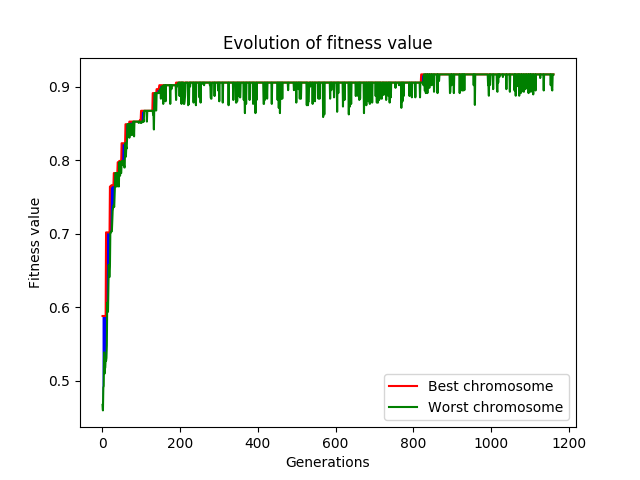
\includegraphics[scale=0.43]{img/am-best-ionosphere.png}
	\caption{Evolución del mejor y peor cromosoma de la población.}
\end{minipage}%
\begin{minipage}{.5\textwidth}
	\centering
	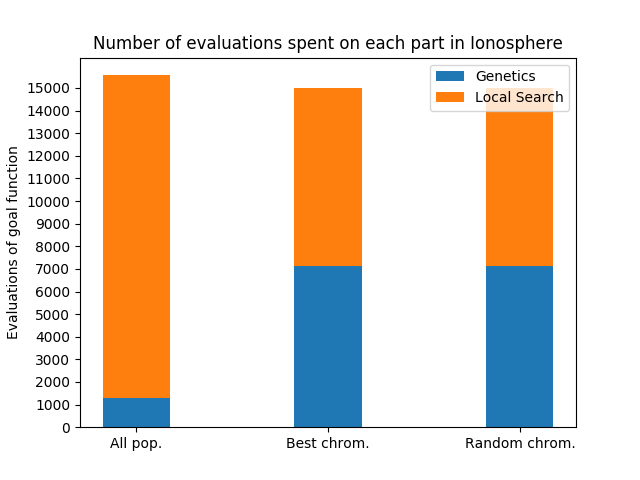
\includegraphics[scale=0.43]{img/bars-ionosphere.png}
	\caption{Comparación entre las evaluaciones en los AM.}
\end{minipage}
\end{figure}

En el gráfico de la izquierda se puede ver como cada vez que se aplica la BL sobre el mejor de la población se producen picos
con respecto al peor cromosoma, es decir, que el valor \textit{fitness} del mejor va mejorando más. Sin embargo, se puede ver
que hay un punto, a partir de cerca de las 200 generaciones que el mejor se estanca, posiblemente debido a que no se produce
ningún hijo mejor, ninguna mutación puede hacerlo mejorar y la BL no encuentra un buen movimiento para él. Sin embargo, casi al
final parece que, posiblemente con algún cruce o mutación se sale de esa zona de estancamiento y se mejora el \textit{fitness}.
En el gráfico de la derecha se puede ver lo que se ha comentado antes. Debido a que hay menos características (32 en este caso),
el número de evaluaciones que realiza la búsqueda local es menor en casi todos los casos (aunque no se note mucho al aplicarla
sobre toda la población, ya que se van a realizar muchas BL). Se puede ver en los otros dos casos (BL sobre el mejor y sobre uno
aleatorio que se aplica el genético aproximadamente un 20\% más que en el conjunto de datos anterior.

Comparando ahora las dos estrategias genéticas, nos encontramos que, de forma nada sorprendente, el AGG con BLX es mejor en
absolutamente todos los aspectos (menos en reducción, donde ambos reducen igual). Esto se puede deber a que o bien se muta más en
el AGG, ya que la mutación se puede aplicar sobre alguno de los 30 cromosomas que han sido generados para sustituir a la población
frente a los 2 posibles nuevos cromosmas, que además no mutan siempre, ya que es más raro que se produzca en este caso; o bien a
que se producen más cruces, y por tanto, el mejor cromosoma tiene más probabilidades de salir en los torneos binarios.
mejor de los casos). Para ver un poco mejor estos algoritmos, veamos las siguientes gráficas:

\begin{figure}[H]
\centering
\begin{minipage}{.5\textwidth}
	\centering
	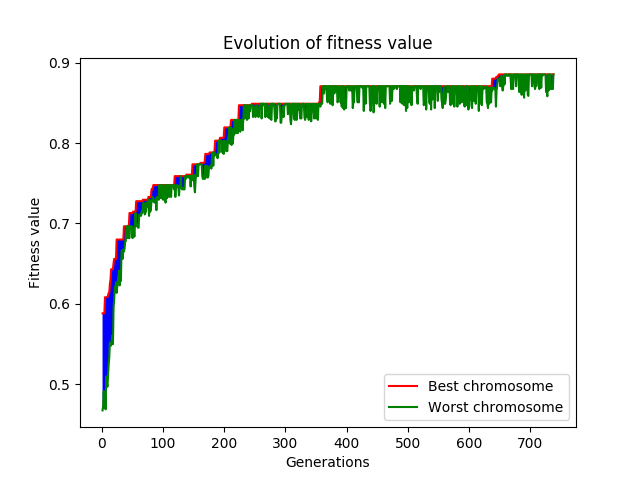
\includegraphics[scale=0.43]{img/agg-blx-ionosphere.png}
	\caption{AGG con BLX.}
\end{minipage}%
\begin{minipage}{.5\textwidth}
	\centering
	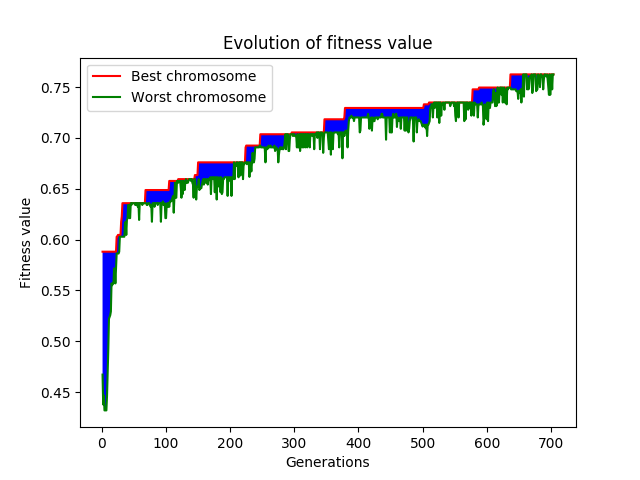
\includegraphics[scale=0.43]{img/agg-ac-ionosphere.png}
	\caption{AGG con cruce aritmético.}
\end{minipage}
\end{figure}

\begin{figure}[H]
\centering
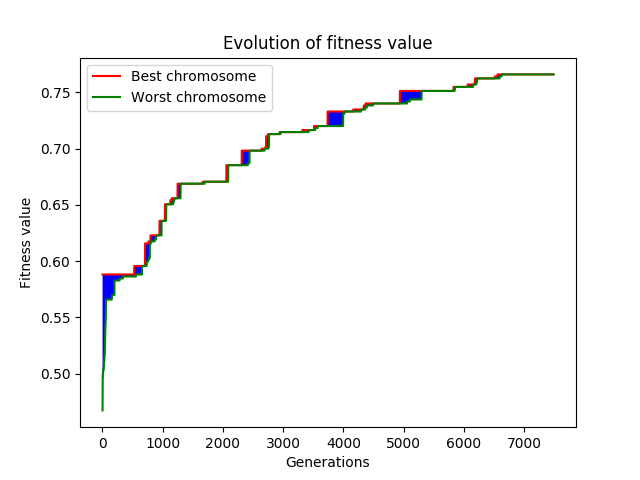
\includegraphics[scale=0.6]{img/age-ac-ionosphere.png}
\caption{AGE con cruce aritmético.}
\end{figure}

Como se puede ver, de nuevo, el AGG con BLX crece más, pero también se estanca más a menudo, ya que no se produce ninguna mejora
durante muchas generaciones a partir de las 200. El AGG con CA no se estanca tanto, pero deja una mayor diferencia entre el
mejor y el peor, con lo cuál, la población no converge tanto hacia el mejor cromosoma, cosa que pasaba en el caso contrario.
En el AGE con CA se puede ver como casi toda la polación converge muy rápidamente, pero que sin embargo sigue mejorando, aunque
sea de forma un poco más lenta. Es por eso qu posiblemente sea peor que el AGE con BLX, ya que al hacer la media, como se ha
dicho antes, se tiende a que se equilibren más los cromosomas a valores medios, con lo cuál se reduce la disparidad entre los
extremos de la población.

Comparando los AG y los AM ganadores, podemos ver que claramente el mejor de ellos es el AM con BL sobre el mejor de la población,
ya que comparándolo con el mejor genético (el AGG con BLX), se puede ver que es muy superior a este en todos los valores medios.
Con lo cuál, tenemos otra victoria de los meméticos sobre los genéticos, lo cuál parece ir indicando que es una buena idea
hibridar las filosofía de exploración de los genéticos con la filosofía de explotación de los meméticos.

Y ahora, comparando todos los resultados medios, podemos ver que el ganador absoluto de nuevo es el \textbf{AM con BL sobre el
mejor}. Se puede ver como clasifica mucho mejor que las técnicas estudiadas en la práctica anterior, como reduce un poco menos
que la BL a secas, pero como en la agrupación es capaz de ganarla de forma significativa (estamos hablando de casi del 2\% de
mejora). Comparar el tiempo no sería muy justo, ya que el AM es una búsqueda basada en poblaciones mientras que la otra es una
búsqueda basada en trayectorias. Sin embargo, aquí podemos ver que la BL de la que partimos para constuir los meméticos
es bastante buena, ya que hibridándola con los AG nos da muy buenos resultados.

Pasemos ahora a estudiar el último conjunto de datos, \textit{Texture}, y comencemos de nuevo con los AGG. De nuevo, y para
sorpresa de nadie, el AGG con cruce BLX es mejor en casi todos los aspectos que su rival, el AGG con CA, menos en tasa de
clasificación, donde es un poco peor (aproximadamente un 2\% inferior). Pero, debido a que reduce más, es capaz de obetener
una mayor tasa de reducción y una mejor agrupación, siendo capaz, por tanto, de a lo mejor generalizar mejor que el AGG con CA
en caso de disponer de más datos.

Pasando a analizar ahora a estudiar los AGE, nos encontramos de nuevo que el mejor es el AGE con BLX y, a diferencia de los AGG
para este conjunto de datos, nos encontramos que aquí el BLX domina sobre el CA en todos los aspectos, haciéndolo por tanto muy
superior al otro, por los motivos ya comentados anteriormente (la media tiende a equilibrar más la población, en este caso, los
pocos descendientes que se generan, los cuáles son los únicos capaces de mejorar la población).

Estudiando el caso de los AM, nos encontramos ante un caso difícil, ya que los 3 algoritmos dan muy buenos resultados. El AM que
aplica la BL sobre toda la población ofrece una mejor tasa de clasificación, pero en cuanto a reducción es el que peor va. El AM
que aplica la BL sobre el mejor es el que tarda menos y ofrece una mejor tasa de reducción, pero en cuanto a clasificación se ve
superado por el anterior y en agrupación no es tan bueno. Con lo cuál, solo nos queda uno: el AM que aplica la BL sobre un
cromosoma aleatorio. Este es el algoritmo que ofrece la mejor tasa de agrupación, con lo cuál es la técnica más equilibrada, ya
que clasifica de media muy bien (mejor que el que aplica la BL sobre el mejor) y reduce de media mejor que el que aplica la BL 
sobre toda la población, con lo cuál, con unos resultados tan equilibrados, es el que podría llegar a tener mejores resultados
si dispusiéramos de más datos para probar. Así que, debido a lo equilibrado que es, vamos a quedarnos con el AM que aplica la BL
sobre un cromosoma aleatorio.

Para ver un poco mejor a estos algoritmos, vamos a ver algunas gráficas que comparan el AM que aplica la BL sobre toda la
población, el que la aplica sobre un cromosoma aleatorio y los gráficos de barras de la cantidad de evaluaciones que se utilizan
en la BL y en el genético:

\begin{figure}[H]
\centering
\begin{minipage}{.5\textwidth}
	\centering
	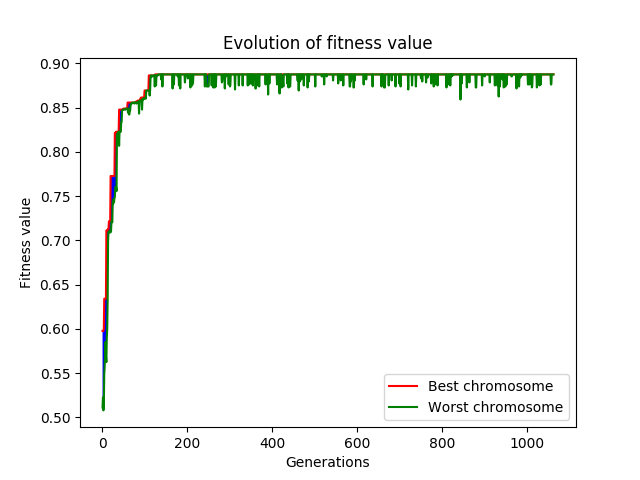
\includegraphics[scale=0.43]{img/am-rand-texture.png}
	\caption{AM con BL sobre un cromosoma aleatorio.}
\end{minipage}%
\begin{minipage}{.5\textwidth}
	\centering
	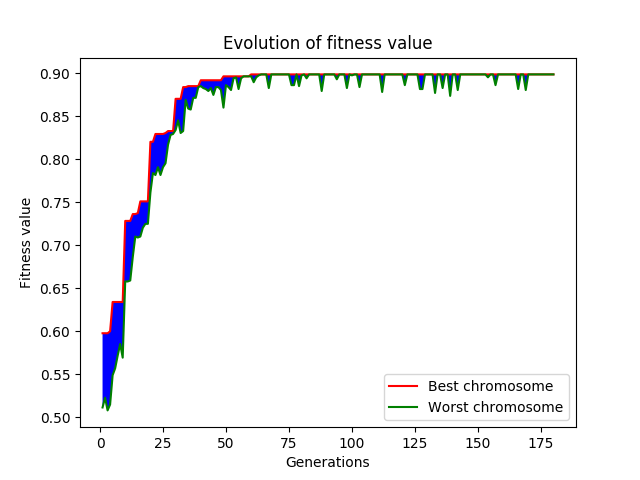
\includegraphics[scale=0.43]{img/am-all-texture.png}
	\caption{AM con BL sobre un toda la población.}
\end{minipage}
\end{figure}

\begin{figure}[H]
\centering
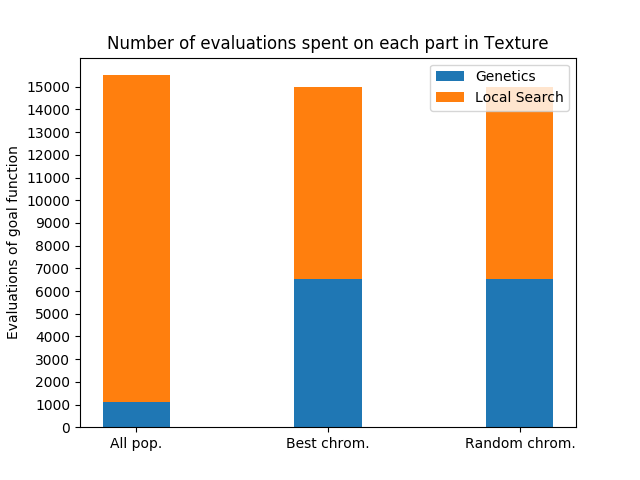
\includegraphics[scale=0.6]{img/bars-texture.png}
\caption{Comparación entre las evaluaciones en los AM.}
\end{figure}

Se puede ver como el que aplica la BL sobre un cromosoma aleatorio llega más rápido a su óptimo, y por tanto, es el que más rápido
converge de los dos, y se puede ver como el peor cromosoma va cambiando mucho mientras que el mejor ya ha llegado a un óptimo
local. El que aplica BL sobre toda la población hace que el \textit{fitness} del mejor y peor crezca de una forma más equilibrada
hasta que llega al punto de convergencia, donde el mejor se estanca mientras que el peor va variando y se puede ver que la
distancia entre ellos va creciendo o decreciendo según qué generación sea. Y, observando el gráfico de barras, podemos ver que,
como pasaba en el conjunto de datos anterior, las evaluaciones de la BL y el AG más o menos se equilibran cuando se aplica la BL
sobre un cromosoma aleatorio o el mejor, mientras que en el otro caso se sigue evaluando poco el genético. Sin embargo, a
diferencia del caso anterior, se ve como se reduce un poco el número de evaluaciones del genético en todos los casos, ya que
esta vez hay más características, con lo cuál, se aplica un poco más la BL que el caso anterior.

Evaluando ahora el mejor genético, nos encontramos que de nuevo el mejor es el AGG con BLX, ya que, a pesar de ofrecer de media
una tasa de clasificación un poco peor, nos encontramos que reduce más, tiene una mayor agrupación y un menor tiempo, con lo
cuál lo hace preferible sobre su homónimo con otro criterio.

Las siguientes gráficas ayudan a ver esta idea:

\begin{figure}[H]
\centering
\begin{minipage}{.5\textwidth}
	\centering
	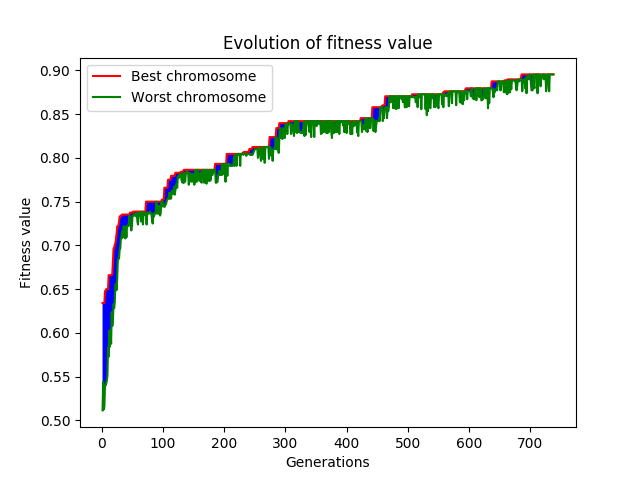
\includegraphics[scale=0.43]{img/agg-blx-texture.png}
	\caption{AGG con BLX.}
\end{minipage}%
\begin{minipage}{.5\textwidth}
	\centering
	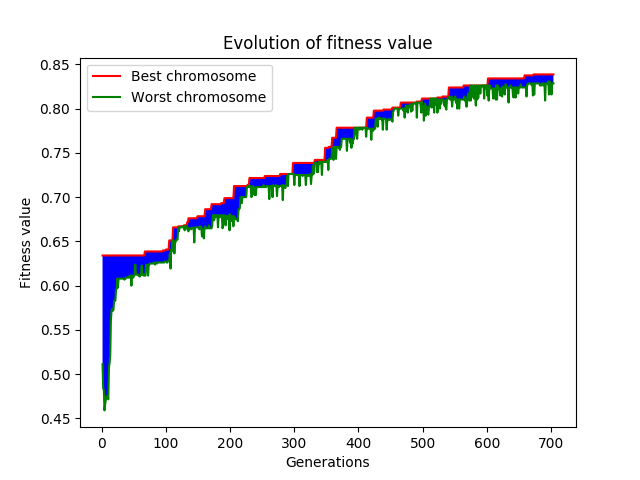
\includegraphics[scale=0.43]{img/agg-ac-texture.png}
	\caption{AGG con cruce aritmético.}
\end{minipage}
\end{figure}

\begin{figure}[H]
\centering
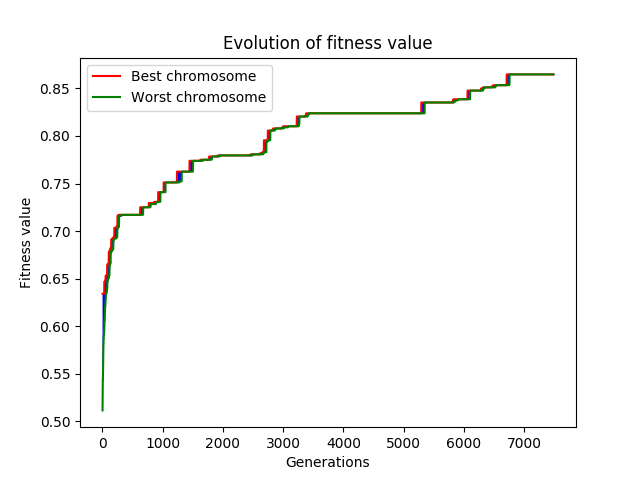
\includegraphics[scale=0.6]{img/age-blx-texture.png}
\caption{AGE con BLX.}
\end{figure}

Como se puede ver, de nuevo, el AGG con BLX es donde más crece el mejor valor y se puede ver como la diferencia entre el mejor
y el peor se va haciendo cada vez más y más sutil. En el caso del AGG con CA, se puede ver como hay un poco más de variabilidad,
posiblemente porque en ese conjunto de datos no se consigue que toda la población converja al mejor cromosoma, si no que hay
un poco más de variedad. En cuanto al AGE con BLX, se puede ver como los valores \textit{fitness} del mejor y el peor van
mejorando, pero que la población ha convergido desde muy pronto, ya que a penas hay diferencia entre los dos extremos.

Analizando ahora la mejor metaheurística, nos encontramos que el AM con BL sobre un cromosoma aleatorio es mejor en casi todos
los sentidos que el AGG con BLX, menos en tasa de clasificación, donde es un poco inferior. Sin embargo, le gana en todos los
otros aspectos, siendo esto de nuevo una victoria de los meméticos sobre los genéticos, mostrándonos que es una muy buena idea
el hibridar algoritmos que exploran mucho como pueden ser los AG con algoritmos que explotan mucho, como puede ser la BL.

Comparando ahora la mejor metaheurística con el resto de algoritmos nos encontramos que, en este caso, nuestro AM produce unas
tasas de clasificación mucho peores que por ejemplo el \textit{RELIEF}, el 1-NN o la BL. Si comparamos el AM con la BL, podemos
ver que, no obstante, nuestra metaheurística ofrece unos mejores valores medios que la BL en general, menos en la tasa de
clasificación. Por tanto, si nos atendiésemos a este criterio, podemos decir que el AM es mucho mejor que la BL, ya que se puede
dar el caso de que generalice mejor luego, o que posiblemente haya alguna partición que reduzca mucho la tasa de clasificación,
como sucede en este caso. Si nos atendemos solamente a la tasa de clasificación, el mejor sería el \textbf{\textit{RELIEF}}, 
pero como este no es capaz de reducir, nadie nos dice que con nuevas particiones o más datos sea capaz de tener un rendimiento
inferior. Sin embargo esto es un indicativo de que el algoritmo greedy que tenemos es muy bueno, y que por tanto merece la pena
intentar combinarlo con nuestras metaheurísticas, que es lo que se propone a continuación, con el objetivo de ver si se produce
alguna mejora.

\subsection{Experimentación}

En este breve apartado vamos a intentar combinar el AGG con BLX y el AM con BL sobre el mejor cromosoma junto con el
\textit{RELIEF} para intentar mejorar nuestros resultados.

Lo que se ha hecho es inicializar una población con la solución obtenida por \textit{RELIEF} modificando un 25\% de los genes
de cada cromosoma de forma aleatoria. Es decir, se ha intentado hacer una especie de GRASP, ya que se ha partido del greedy,
se ha obtenido una población con él y se ha modificado de forma aleatoria cada cromosoma de la población para introducir
diversidad en ésta.

Los resultados obtenidos se pueden ver en las siguientes tablas:


\begin{table}[H]
\resizebox{\columnwidth}{!}{%
\begin{tabular}{c|c|c|c|c|c|c|c|c|c|c|c|c|}
\cline{2-13}
                                            & \multicolumn{4}{c|}{\textbf{Colposcopy}}                                 & \multicolumn{4}{c|}{\textbf{Ionosphere}}                        & \multicolumn{4}{c|}{\textbf{Texture}}                           \\ \cline{2-13} 
                                            & \textit{\textbf{\%\_clas}} & \textit{\textbf{\%red}} & \textit{\textbf{Agr.}} & \textbf{T} & \textit{\textbf{\%\_clas}} & \textit{\textbf{\%red}} & \textit{\textbf{Agr.}} & \textbf{T} & \textit{\textbf{\%\_clas}} & \textit{\textbf{\%red}} & \textit{\textbf{Agr.}} & \textbf{T} \\ \hline
\multicolumn{1}{|c|}{\textbf{Partición 1}}  & 76.27             & 79.03                   & 77.65         & 8.34       & 94.37             & 85.29          & 89.83         & 6.67       & 90.91             & 85.0           & 87.95         & 6.32       \\ \hline
\multicolumn{1}{|c|}{\textbf{Partición 2}}  & 77.19             & 77.42                   & 77.31         & 9.16       & 84.29             & 82.35          & 83.32         & 6.64       & 90.0              & 77.5           & 83.75         & 6.12       \\ \hline
\multicolumn{1}{|c|}{\textbf{Partición 3}}  & 78.95             & 80.65                   & 79.8          & 6.61       & 92.86             & 85.29          & 89.08         & 6.5        & 90.0              & 82.5           & 86.25         & 5.93       \\ \hline
\multicolumn{1}{|c|}{\textbf{Partición 4}}  & 73.68             & 82.26                   & 77.97         & 5.82       & 90.0              & 91.18          & 90.59         & 6.06       & 89.09             & 80.0           & 84.55         & 6.2        \\ \hline
\multicolumn{1}{|c|}{\textbf{Partición 5}}  & 75.44             & 80.65                   & 78.04         & 8.27       & 90.0              & 70.59          & 80.29         & 9.05       & 85.45             & 82.5           & 83.98         & 6.56       \\ \hline
\multicolumn{1}{|c|}{\textbf{Media}}        & 76.31             & 80.0                    & 78.15         & 7.64       & 90.3              & 82.94          & 86.62         & 6.98       & 89.09             & 81.5           & 85.3          & 6.23       \\ \hline
\multicolumn{1}{|c|}{\textbf{Máximo}}       & 78.95             & 82.26                   & 79.8          & 9.16       & 94.37             & 91.18          & 90.59         & 9.05       & 90.91             & 85.0           & 87.95         & 6.56       \\ \hline
\multicolumn{1}{|c|}{\textbf{Mínimo}}       & 73.68             & 77.42                   & 77.31         & 5.82       & 84.29             & 70.59          & 80.29         & 6.06       & 85.45             & 77.5           & 83.75         & 5.93       \\ \hline
\multicolumn{1}{|c|}{\textbf{Mediana}}      & 76.27             & 80.65                   & 77.97         & 8.27       & 90.0              & 85.29          & 89.08         & 6.64       & 90.0              & 82.5           & 84.55         & 6.2        \\ \hline
\multicolumn{1}{|c|}{\textbf{Desv. Típica}} & 1.75              & 1.64                    & 0.86          & 1.23       & 3.45              & 6.81           & 4.07          & 1.06       & 1.91              & 2.55           & 1.59          & 0.21       \\ \hline
\end{tabular}
}%
\caption{Resultados obtenidos por el AGG con cruce BLX-$\alpha$ y población inicial obtenida por \textit{RELIEF} en el problema
del APC.}
\end{table}

\begin{table}[H]
\resizebox{\columnwidth}{!}{%
\begin{tabular}{c|c|c|c|c|c|c|c|c|c|c|c|c|}
\cline{2-13}
                                            & \multicolumn{4}{c|}{\textbf{Colposcopy}}                                 & \multicolumn{4}{c|}{\textbf{Ionosphere}}                        & \multicolumn{4}{c|}{\textbf{Texture}}                           \\ \cline{2-13} 
                                            & \textit{\textbf{\%\_clas}} & \textit{\textbf{\%red}} & \textit{\textbf{Agr.}} & \textbf{T} & \textit{\textbf{\%\_clas}} & \textit{\textbf{\%red}} & \textit{\textbf{Agr.}} & \textbf{T} & \textit{\textbf{\%\_clas}} & \textit{\textbf{\%red}} & \textit{\textbf{Agr.}} & \textbf{T} \\ \hline
\multicolumn{1}{|c|}{\textbf{Partición 1}}  & 71.19             & 82.26                   & 76.72         & 5.97       & 83.1              & 88.24          & 85.67         & 3.15       & 87.27             & 87.5           & 87.39         & 3.86       \\ \hline
\multicolumn{1}{|c|}{\textbf{Partición 2}}  & 64.91             & 82.26                   & 73.59         & 6.04       & 85.71             & 88.24          & 86.97         & 3.27       & 86.36             & 85.0           & 85.68         & 4.46       \\ \hline
\multicolumn{1}{|c|}{\textbf{Partición 3}}  & 75.44             & 87.1                    & 81.27         & 4.21       & 80.0              & 91.18          & 85.59         & 3.39       & 92.73             & 85.0           & 88.86         & 4.78       \\ \hline
\multicolumn{1}{|c|}{\textbf{Partición 4}}  & 80.7              & 85.48                   & 83.09         & 4.65       & 92.86             & 82.35          & 87.61         & 4.36       & 92.73             & 85.0           & 88.86         & 4.62       \\ \hline
\multicolumn{1}{|c|}{\textbf{Partición 5}}  & 73.68             & 87.1                    & 80.39         & 4.62       & 87.14             & 88.24          & 87.69         & 3.37       & 84.55             & 85.0           & 84.77         & 4.32       \\ \hline
\multicolumn{1}{|c|}{\textbf{Media}}        & 73.18             & 84.84                   & 79.01         & 5.09       & 85.76             & 87.65          & 86.7          & 3.51       & 88.73             & 85.5           & 87.11         & 4.41       \\ \hline
\multicolumn{1}{|c|}{\textbf{Máximo}}       & 80.7              & 87.1                    & 83.09         & 6.04       & 92.86             & 91.18          & 87.69         & 4.36       & 92.73             & 87.5           & 88.86         & 4.78       \\ \hline
\multicolumn{1}{|c|}{\textbf{Mínimo}}       & 64.91             & 82.26                   & 73.59         & 4.21       & 80.0              & 82.35          & 85.59         & 3.15       & 84.55             & 85.0           & 84.77         & 3.86       \\ \hline
\multicolumn{1}{|c|}{\textbf{Mediana}}      & 73.68             & 85.48                   & 80.39         & 4.65       & 85.71             & 88.24          & 86.97         & 3.37       & 87.27             & 85.0           & 87.39         & 4.46       \\ \hline
\multicolumn{1}{|c|}{\textbf{Desv. Típica}} & 5.18              & 2.19                    & 3.42          & 0.76       & 4.3               & 2.88           & 0.91          & 0.43       & 3.38              & 1.0            & 1.66          & 0.31       \\ \hline
\end{tabular}
}%
\caption{Resultados obtenidos por el AM con cruce BLX-$\alpha$, población inicial obtenida por \textit{RELIEF} y Búsqueda Local
sobre un cromosoma aleatorio  de la población en el problema del APC.}
\end{table}

\begin{table}[H]
\resizebox{\columnwidth}{!}{%
\begin{tabular}{c|c|c|c|c|c|c|c|c|c|c|c|c|}
\cline{2-13}
                                                       & \multicolumn{4}{c|}{\textbf{Colposcopy}}                                 & \multicolumn{4}{c|}{\textbf{Ionosphere}}                        & \multicolumn{4}{c|}{\textbf{Texture}}                           \\ \cline{2-13} 
                                                       & \textit{\textbf{\%\_clas}} & \textit{\textbf{\%red}} & \textit{\textbf{Agr.}} & \textbf{T} & \textit{\textbf{\%\_clas}} & \textit{\textbf{\%red}} & \textit{\textbf{Agr.}} & \textbf{T} & \textit{\textbf{\%\_clas}} & \textit{\textbf{\%red}} & \textit{\textbf{Agr.}} & \textbf{T} \\ \hline
\multicolumn{1}{|c|}{\textbf{1-NN}}                    & 74,88             & 0                       & 37,44         & 0.00039    & 86,33             & 0              & 43,16         & 0.00039    & 92,36             & 0              & 46,18         & 0.00049    \\ \hline
\multicolumn{1}{|c|}{\textbf{RELIEF}}                  & 74,23             & 39,35                   & 56,79         & 0.03659    & 88,89             & 2,94           & 45,92         & 0.03987    & 94,91             & 7,50           & 51,20         & 0.08739    \\ \hline
\multicolumn{1}{|c|}{\textbf{BL}}                      & 72,06             & 81,29                   & 76,68         & 2.73476    & 86,32             & 88,24          & 87,28         & 0.67943    & 91,09             & 82,50          & 86,80         & 1.09861    \\ \hline
\multicolumn{1}{|c|}{\textbf{AGG-BLX}}                 & 74.54             & 70.32                   & 72.43         & 11.1       & 85.48             & 85.29          & 85.39         & 4.78       & 89.82             & 82.5           & 86.16         & 6.47       \\ \hline
\multicolumn{1}{|c|}{\textbf{AGG-CA}}                  & 74.52             & 53.55                   & 64.03         & 17.35      & 87.18             & 64.71          & 75.94         & 9.48       & 91.82             & 67.5           & 79.66         & 9.88       \\ \hline
\multicolumn{1}{|c|}{\textbf{AGE-BLX}}                 & 71.79             & 71.94                   & 71.86         & 11.81      & 84.03             & 85.29          & 84.66         & 6.59       & 90.91             & 77.0           & 83.95         & 8.2        \\ \hline
\multicolumn{1}{|c|}{\textbf{AGE-CA}}                  & 71.76             & 66.45                   & 69.1          & 13.54      & 86.61             & 67.06          & 76.84         & 10.46      & 89.82             & 72.0           & 80.91         & 10.03      \\ \hline
\multicolumn{1}{|c|}{\textbf{AM-(10,1.0)}}             & 76.35             & 83.55                   & 79.95         & 7.7        & 82.63             & 90.0           & 86.31         & 3.68       & 90.73             & 84.0           & 87.36         & 5.32       \\ \hline
\multicolumn{1}{|c|}{\textbf{AM-(10,0.1)}}             & 73.87             & 83.23                   & 78.55         & 6.14       & 86.03             & 88.82          & 87.43         & 3.22       & 89.27             & 86.0           & 87.64         & 4.52       \\ \hline
\multicolumn{1}{|c|}{\textbf{AM-(10,0.1mej)}}          & 70.01             & 82.9                    & 76.46         & 7.17       & 90.31             & 87.65          & 88.98         & 3.44       & 88.18             & 86.5           & 87.34         & 4.39       \\ \hline
\multicolumn{1}{|c|}{\textbf{AGG-BLX + RELIEF}}        & 76.31             & 80.0                    & 78.15         & 7.64       & 90.3              & 82.94          & 86.62         & 6.98       & 89.09             & 81.5           & 85.3          & 6.23       \\ \hline
\multicolumn{1}{|c|}{\textbf{AM-(10,0.1mej) + RELIEF}} & 73.18             & 84.84                   & 79.01         & 5.09       & 85.76             & 87.65          & 86.7          & 3.51       & 88.73             & 85.5           & 87.11         & 4.41       \\ \hline
\end{tabular}
}%
\caption{Valores medios de los distintos algoritmos más los algoritmos modificados para el problema del APC.}
\end{table}

Vamos a relizar un estudio breve para cada conjunto de datos para ver si se produce o no mucha mejora y si merece la pena intentar
implementarlo o no.

En el conjunto de datos \textit{Colposcopy} nos encontramos que el AM con \textit{RELIEF} no consigue muy buenos resultados,
ya que se queda muy por detrás del mejor algoritmo de ese conjunto de datos. El AGG-BLX con \textit{RELIEF}, sin embargo, si
que ha sufrido una importante mejora, ya que se queda muy cerca en tasa de clasficación y agrupación media respecto al mejor AM,
mientras que baja en tasa de reducción y el tiempo es ligeramente superior al mejor AM. Con lo cuál, en este caso, podemos ver
que ha supuesto una buena mejora sobre el AGG con BLX que ya había anteriormente, ya que lo mejora con creces, y se queda
relativamente cerca del mejor algoritmo.

A continuación se muetran algunas gráficas de como evolucionan los dos algoritmos nuevos:

\begin{figure}[H]
\centering
\begin{minipage}{.5\textwidth}
	\centering
	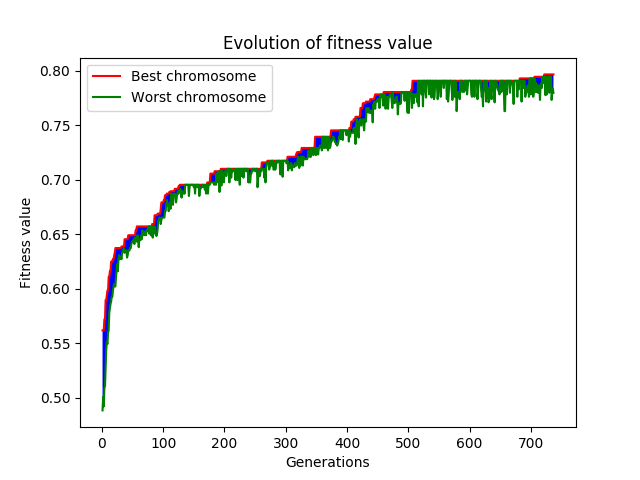
\includegraphics[scale=0.43]{img/agg-blx-relief-colposcopy.png}
	\caption{AGG con BLX y población inicializada con \textit{RELIEF} aleatorio.}
\end{minipage}%
\begin{minipage}{.5\textwidth}
	\centering
	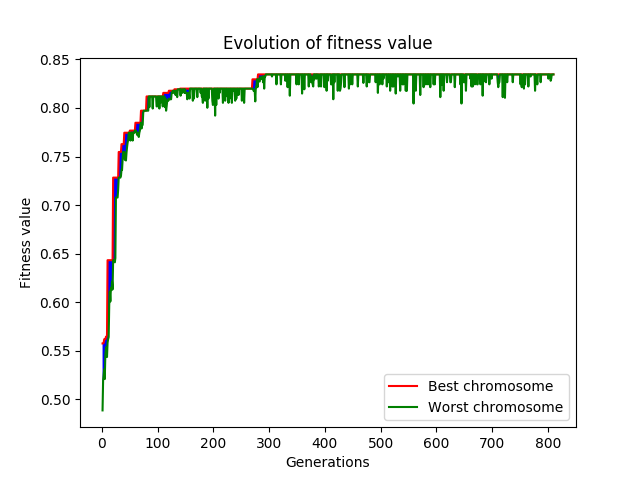
\includegraphics[scale=0.43]{img/am-best-relief-colposcopy.png}
	\caption{AM con BL sobre el mejor y población inicializada con \textit{RELIEF} aleatorio.}
\end{minipage}
\end{figure}

Se puede ver como en el caso del genético casi no se estanca, ya que hay más diversidad, mientras que en el caso del memético
sí que se estanca el mejor y lo hace relativamente pronto.

Pasemos ahora al conjunto de datos \textit{Ionosphere}. Aquí sucede algo similar. El AM con \textit{RELIEF} no es capaz de
tener unos buenos resultados medios, mientras que el AGG con \textit{RELIEF} gana al AGG con BLX normal en tasa de clasificación
y agrupación, pero baja un poco en reducción y empeora un poco el tiempo. Sin embargo, como no estamos considerando mucho el
tiempo, se puede decir que mejora con creces a los AGG. Y de nuevo, como en el caso anterior, se queda muy cerca del mejor
algoritmo, el AM con BL sobre el mejor. Es un poco peor que el mejor algoritmo, pero es capaz de ofrecer unos resultados
muy buenos.

A continuación se muetran algunas gráficas para ver los nuevos algoritmos en acción:

\begin{figure}[H]
\centering
\begin{minipage}{.5\textwidth}
	\centering
	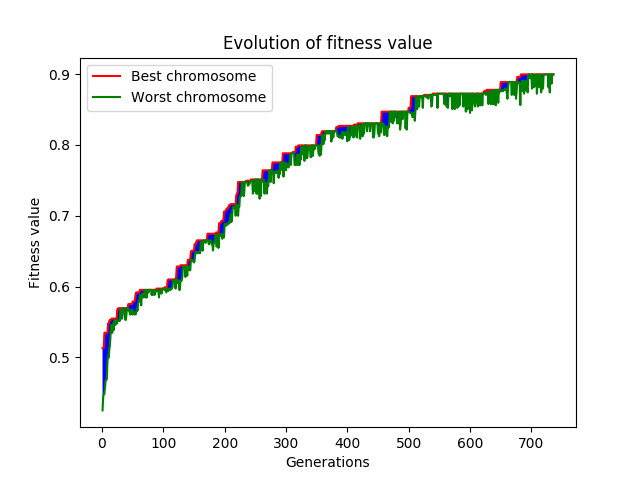
\includegraphics[scale=0.43]{img/agg-blx-relief-ionosphere.png}
	\caption{AGG con BLX y población inicializada con \textit{RELIEF} aleatorio.}
\end{minipage}%
\begin{minipage}{.5\textwidth}
	\centering
	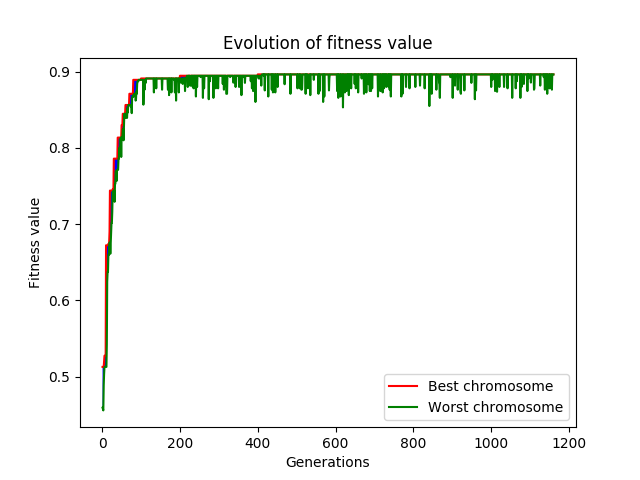
\includegraphics[scale=0.43]{img/am-best-relief-ionosphere.png}
	\caption{AM con BL sobre el mejor y población inicializada con \textit{RELIEF} aleatorio.}
\end{minipage}
\end{figure}

Aquí, como en el caso anterior, el AGG con \textit{RELIEF} crece mucho casi sin estancarse, lo cuál explicaría sus buenos
resultados. Sin embargo, el AM con \textit{RELIEF} se estanca muy rápido en un óptimo local y no es capaz de mejorar nada, lo
cuál explicaría sus malos resultados.

Finalmente, llegamos de nuevo al conjunto de datos \textit{Texture}. Aquí, sin embargo, nuestra nueva implementación resulta
insatisfactoria, ya que no hemos obtenido ninguna mejora respecto a la mejor metaheurística, el AM con BL sobre un cromosoma
aleatorio, por no decir que en cuanto a tasas de clasificación se refiere nuestros nuevos algoritmos se han quedado
muy lejos del \textit{RELIEF} original. El AGG con \textit{RELIEF} no se acerca al mejor genético, el AGG con BLX (solo en tasa
de clasificación, pero en el resto baja). El AM con \textit{RELIEF} es el peor AM, ya que es el que ofrece peores valores medios.

A continuación se pueden ver algunas gráficas de estos dos algoritmos:

\begin{figure}[H]
\centering
\begin{minipage}{.5\textwidth}
	\centering
	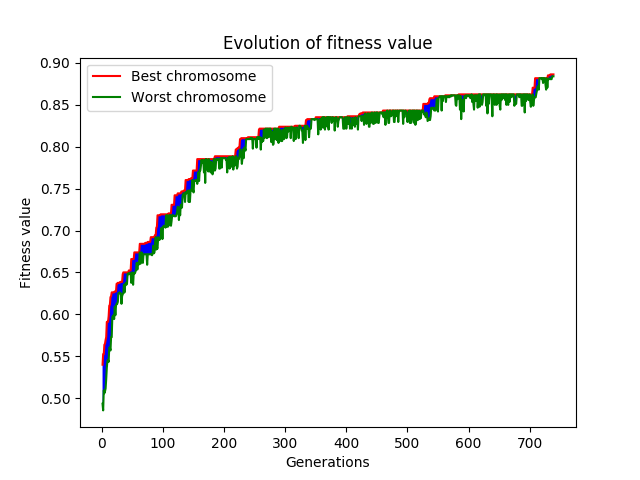
\includegraphics[scale=0.43]{img/agg-blx-relief-texture.png}
	\caption{AGG con BLX y población inicializada con \textit{RELIEF} aleatorio.}
\end{minipage}%
\begin{minipage}{.5\textwidth}
	\centering
	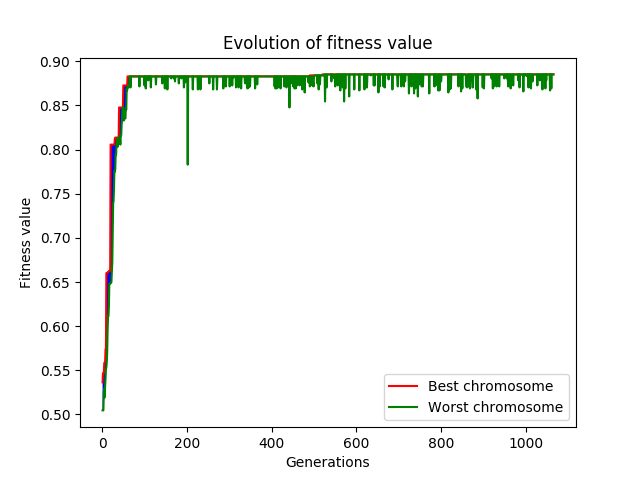
\includegraphics[scale=0.43]{img/am-best-relief-texture.png}
	\caption{AM con BL sobre el mejor y población inicializada con \textit{RELIEF} aleatorio.}
\end{minipage}
\end{figure}

Relativamente hablando, el AGG con \textit{RELIEF} no se estanca, pero su valor \textit{fitness} no crece lo suficiente como
en los casos anteriores. El AM con \textit{RELIEF} se estanca igual de rápido que en el conjunto de datos anterior, lo cuál
explicaría su mal comportamiento.

Como pequeña conclusión, nuestra pequeña versión de GRASP ha mejorado los algoritmos genéticos en los dos primeros
conjuntos de datos, pero en el último no lo suficiente. Sin embargo, de media ha empeorado nuestros algoritmos meméticos, ya que
no tienen los mismos resultados que antes, con lo cuál, en el caso de los meméticos, es mejor no mezclar demasiadas técnicas, ya
que de antes ya teníamos un genético y un memético. Para no dejar un tan mal sabor de boca, podemos decir que es una idea
interesante ofrecer una población generada por un greedy y luego modificar componentes aleatorios de ésta a un AG, ya que con
su capacidad de exploración, y con la diversidad de las soluciones iniciales, puede que sea capaz de explorar el espacio
mucho mejor que generando al población inicial de forma aleatoria pura (se puede ver como el AGG con esta técnica llega a
acercarse en cuanto a resultados a los mejores meméticos, con lo cuál no es un mal punto de partida).

\subsection{Conclusión}

Como conclusión a nuestro análisis general, podemos ver que las técnicas que hemos implementado en esta práctica han dado unos
resultados bastante buenos. 

Por una parte, los algoritmos genéticos nos han permitido explorar el espacio de soluciones de una forma efectiva
en busca de una mejor solución. Por lo general, el esquema generacional ha ofrecido unos mejores resultados que el estacionario,
ya que ha sido capaz de meter mayor diversidad al proceso de búsqueda al permitir más cruces y mutaciones, con lo cuál,
se puede tener una población más diversa y dispersa siempre y cuando se tengan \textbf{suficientes datos}. El elitismo, como
hemos podido ver, es una técnica muy interesante para intentar mantener la mejor solución actual en los AGG con tal de no
perderla, ya que en caso de no haberla aplicado, posiblemente los resultados medios obtenidos hubiesen sido peores, ya que
no se garantizaría la conservación del mejor cromosoma encontrado hasta el momento.

Por otro lado, los algoritmos meméticos nos han mostrado que combinar los buenos resultados que ya daban los algoritmos genéticos
y su capacidad explorativa con los también relativamente buenos resultados que nos daba la búsqueda local y su capacidad
explotativa ha sido una buena idea, ya que nos ha permitido obtener unas soluciones muy buenas en casi todos los conjuntos
de datos de los que disponíamos (menos en el último, donde si se comparase solamente la tasa de clasificación ganaría de nuevo
\textit{RELIEF}). Sin embargo, no hemos podido demostrar cuál es el mejor memético, ya que cada versión ha dado unos buenos
resultados en unos conjuntos de datos y un poco peores en otros. Por tanto, de aquí podemos extraer que lo importante sería
probar las tres técnicas que se han sugerido con el problema concreto y quedarnos con aquella que ofrezca unos mejores resultados,
ya que cada problema es un mundo y no existe una metaheurística general que resuelva todos nuestros problemas de la mejor manera
posible.

Para terminar, como conclusión final podemos decir que las metaheurísticas han ofrecido unos buenos resultados, y que a la hora
de enfrentarnos con un problema de verdad, no debemos dudar en probar diversas técnicas y en escoger \textbf{aquella 
metaheurística que mejor se adapte a nuestro problema}, es decir, la que nos permita obtener los mejores resultados. 

\newpage

\begin{thebibliography}{5}

\bibitem{pykdtree}
Repositroio de GitHub de pykdtree.
\\\url{https://github.com/storpipfugl/pykdtree}

\bibitem{ckdtree}
Documentación de cKDTree.
\\\url{https://docs.scipy.org/doc/scipy/reference/generated/scipy.spatial.cKDTree.html}

\end{thebibliography}

\end{document}

